
\chapter{Experiments} % Main chapter title

\section{Training Details}

The models are trained on dataset "synthetic-50-5" as mentioned in Chapter \ref{ch:04} with 3000 scenes. Each scene has a depth map with dimension $ 128\times 128 $ in height and width, an image with dimension $ 128\times 128 \times 1 $.  The depth map is converted to 3D vertex map as introduced in Chapter \ref{ch:04}. The light map is calculated based on vertex map and the known light position. We create a tensor in PyTorch that includes vertex map, image and the light direction for each scene and considered it as one training case. Thus 3000 scenes has corresponding 3000 training cases. Each scene has a corresponding ground-truth normal map for loss calculation and the evaluation. 

\begin{figure}[H]
	\centering
	
	\begin{subfigure}[b]{0.24\linewidth}
		
\includegraphics[width=\linewidth]{./Figures/test_scenes/03094.depth0.png}
	\end{subfigure}
	\begin{subfigure}[b]{0.24\linewidth}
		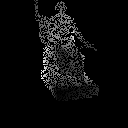
\includegraphics[width=\linewidth]{./Figures/test_scenes/03094.depth0_noise.png}
	\end{subfigure}
	\begin{subfigure}[b]{0.24\linewidth}
		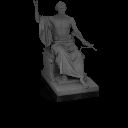
\includegraphics[width=\linewidth]{./Figures/test_scenes/03094.image0.png}
	\end{subfigure}
	\begin{subfigure}[b]{0.24\linewidth}
		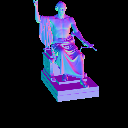
\includegraphics[width=\linewidth]{./Figures/test_scenes/03094.normal0.png}
	\end{subfigure}
	
	
	\begin{subfigure}[b]{0.24\linewidth}
		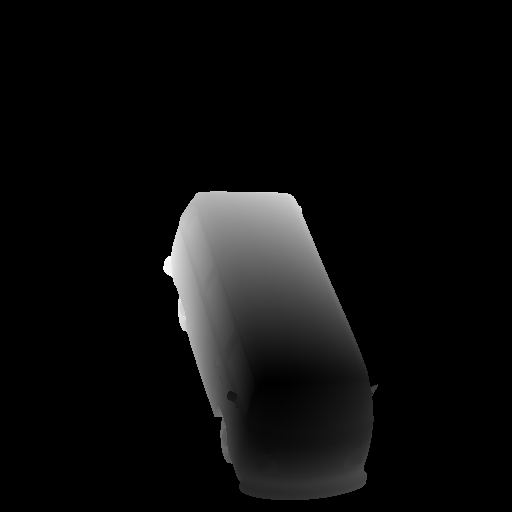
\includegraphics[width=\linewidth]{./Figures/test_scenes/05126.depth0.png}
		\caption{Depth Map}
	\end{subfigure}
	\begin{subfigure}[b]{0.24\linewidth}
		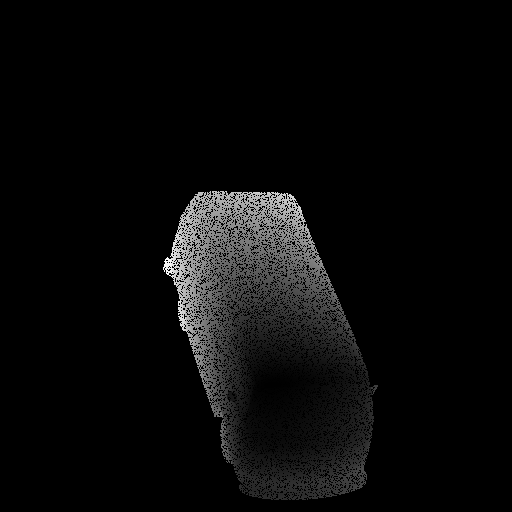
\includegraphics[width=\linewidth]{./Figures/test_scenes/05126.depth0_noise.png}
		\caption{Add noise}
	\end{subfigure}
	\begin{subfigure}[b]{0.24\linewidth}
		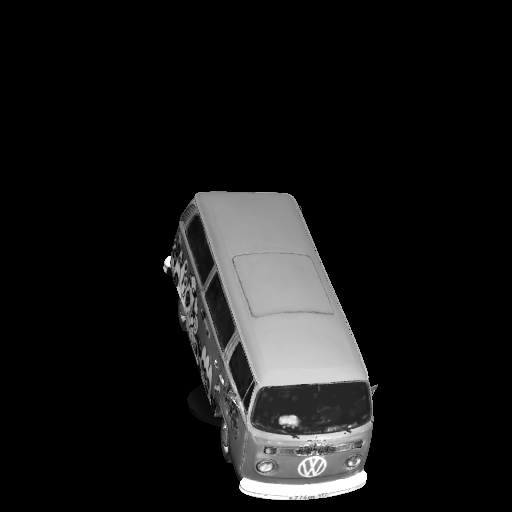
\includegraphics[width=\linewidth]{./Figures/test_scenes/05126.image0.png}
		\caption{Image}
	\end{subfigure}
	\begin{subfigure}[b]{0.24\linewidth}
		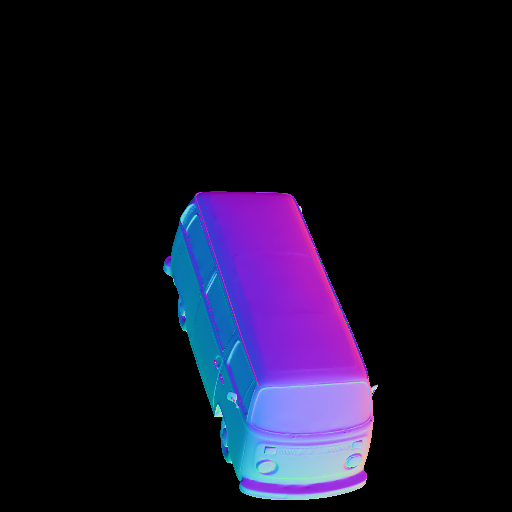
\includegraphics[width=\linewidth]{./Figures/test_scenes/05126.normal0.png}
		\caption{Normal}
	\end{subfigure}
	\decoRule
	\caption{Some of the test scenes during the training. From top to bottom, baoshanlu, Washington, Garfield, Dragon, Bus}
	\label{fig:test-scene}
\end{figure}


The training processes are evaluated in every epochs with 100 evaluation scenes that models never seen before, which contains the 5 different objects in the ``synthetic-50-5" test set. Figure \ref{fig:test-scene} shows some of the test scenes during the training work. Note that the position of objects are not placed always naturally on the stage but with a random rotation in X, Y, Z axes, respectively.

For the training parameters, we set the training pipeline with batch size $ 8 $, we found that a higher batch size will reduce the final performance.  Adam optimizer (\cite{adam}), learning rate start from  $ 1\times10^{-3} $, learning schedule [8,1000], learning decay factor 0.5. The model is trained with PyTorch 1.10.0a0, CUDA 11.4.1, GPU with single NVIDIA GEFORCE RTXA 6000. It takes 14 hours to train GCNN and 35 hours to train the Trip-Net. We terminate the training when the evaluation on the test dataset converged.


GCNN model is the base model of the whole thesis. The architecture is described in \ref{sec:gcnn}. We use a single GCNN to estimate the surface normal based on geometry information. It uses vertex map as input to estimate the corresponding tangent surface normal map. In order to verify the applicability of the skip connection and the gated convolution layers, we trained two extra models as a comparison. The first model, we replace all of the gated layer to standard convolution layers in the network but keeps all of the other settings same, and give it a name ``CNN". It is used to verify the performance the gated convolution layers. As mentioned in chapter \ref{ch:03}, the gated layer is designed to deal with noised input. Since all of the vertex map in the dataset has been added noise, the GCNN is supposed to over-perform ``CNN". 
Another model called ``NOC" is designed to verify the skip connection, which simply removes the skip connections in the network but keeps other settings same. Is is designed to show to which content will skip connection help the model performance. We use Reversed Huber Loss as loss function during the training, since we found it gives a better final error compare to L2 loss. 



\begin{table}[H]
	
	\centering
	\begin{tabular}{l | l l l l l }
		\toprule
		\tabhead{Model} & $ \# $\textbf{Total} &\textbf{ V-P} & \textbf{L-P} & \textbf{I-P} & \tabhead{Size /MB}\\
		\midrule
		\hline
		CNN 					& 17 & 32 & 0 & 0 & 25.5 \\
		\hline
		NOC 					& 32 & 32 & 0 & 0 & 30.6 \\
		\hline
		GCNN 					& 32 & 32 & 0 & 0 & 45.8 \\
		\bottomrule
	\end{tabular}
	\caption{GCNN Model information. Columns V-P, L-P and I-P represent the number of convolution layers in vertex pipe, light pipe and image pipe respectively. Note that one gated convolution layer is constructed with 2 standard layers, thus it is counted as 2. }	
	\label{tab:gcnn-eval-mean}
\end{table}


The Trip-Net model uses three times GCNN architecture with 4 times fusions, which is more difficult to train. It takes the calibrated illuminated RGB-D images as input to estimate the surface normal map. When we train this model, we take the GCNN model as a baseline, to observe the beneficial of illuminated information using with Trip-Net architecture.
Since it is more complicate than GCNN, we also explored the optimum fusion times of the Trip-Net to see any possibility for the model simplification. A set of similar models have been trained with same settings but different fusion times, denotes by Trip-Net-F$ x $, where $ x $ denotes the fusion times. We evaluate the fusion times from 1 to 4. For the learning rate.  we set $ 1e-3 $. It goes well with GCNN model but lead to loss explosion in Trip-Net. Thus we set a learning rate schedule with an extra decay step at epoch 8. The decay factor is $ 0.5$. The batch size is chosen as 8.

We also found that, trip-Net with four times fusion converges obviously faster than fewer fusion times model. However, model F3 with 3 times fusion converge slower than F4 but in the end it achieves a similar evaluation loss with F4(see Qualitative evaluation). The F1 and F2 models are relatively weaker than the other two models. 

However, the sacrifice of accuracy gives a relatively lighter model. Since we remove the fusions between different pipes, the corresponding upsampling layers in the image and light pipes can also be removed. The model can be trained faster and the size is reduced as well. Table \ref{tab:trip-net-size-compare} gives a comparison of the size and training time among different models.


\begin{table}[H]
	
	\centering
	\begin{tabular}{l | l l l l l }
		\toprule
		\tabhead{Model} & $ \# $\textbf{Total} &\textbf{ V-P} & \textbf{L-P} & \textbf{I-P} & \tabhead{Size /MB}\\
		\midrule
		Trip-Net-F1F  			& 88 &  40 & 24 & 24 & 106\\ 
		\hline
		Trip-Net-F2F 			& 92 & 40 & 26 & 26 & 137 \\ 
		\hline
		Trip-Net-F3F 			& 96 & 40 & 28 & 28 & 167 \\
		\hline
		Trip-Net 				& 100 & 40 & 30 & 30 & 198\\
		\bottomrule
	\end{tabular}
	\caption{Trip-Net Model information. Columns V-P, L-P and I-P represent the number of convolution layers in vertex pipe, light pipe and image pipe respectively. Note that one gated convolution layer is constructed with 2 standard layers, thus it is counted as 2. }	
	\label{tab:trip-net-size-compare}
\end{table}


\section{Quantitative Evaluation}
We evaluated our models on synthetic dataset with resolution $ 128\times 128 $. 
Based on metrics proposed by \cite{geometry_based_solution}, 6 different metrics are used for evaluation. Note that the input vertex map is only semi-dense. One of the benefit of GCNN architecture is the robust to the noisy input, thus in the evaluation, all the points including missing points in the input vertex map are taken into account. 

\paragraph{Average Angle Error Metric}
The metric calculate the average angle error for each point between the inferred normal and ground-truth normal. 
\paragraph{Median Angle Error Metric}
The metric calculate the median angle error of all the point in the normal map.
\paragraph{5 Degree Error Metric}
The metric calculate the percentage of the predicted normals that has error less than 5 degrees comparing to ground-truth.
\paragraph{11.5 Degree Error Metric}
The metric calculate the percentage of the predicted normals that has error less than 11.5 degrees comparing to ground-truth.
\paragraph{22.5 Degree Error Metric}
The metric calculate the percentage of the predicted normals that has error less than 22.5 degrees comparing to ground-truth.
\paragraph{30 Degree Error Metric}
The metric calculate the percentage of the predicted normals that has error less than 30 degrees comparing to ground-truth.

We evaluate the trained models on ``synthetic-50-5". 5 objects are considered in the test dataset. They are: $ Baoshanlu $, $ Bus $, $ Dragon $, $ Garfield $, and $ Washington $. Each object has 20 scenes with total 100 scenes for 5 objects. The test objects do not exist in the training dataset. We evaluate all the presented models on the test dataset, in order to fit them in one table, the name of each models are simplified. $ SVD $ model use SVD optimization method, $ NOC $ model is the no skip connection version of $ GCNN $, $ CNN $ is the CNN version of $ GCNN $. $ F1 $, $ F2 $, $ F3 $,$ F4 $ means the fusion times in the Trip-Net. 

When evaluate the $ GCNN $ models, we can take $ SVD $ model as baseline, $ NOC $ and $ CNN $ are used to verify the performance of $ GCNN $ model. When evaluate the $ F1-F4 $ models, we can take $ GCNN $ model as baseline. 

From the table we can see that all the learning based approaches achieves a better result than SVD approach. In the 30 degrees error metric, GCNN based approach achieves 95 \% accuracy whereas Trip-Net is even higher, some of the models like $ dragon $ achieves 98\%. The best performance is around 90\%, 75 \%, 45 \% in $ 22.5^\circ $, $ 11.5^\circ $ and $ 5^\circ $ degrees error metric respectively. Another notable result is the close performance of F3 and F4 models, where they achieves a very comparable performance. We also found that during the training, F4 model converges faster than F3, but F3 in the end achieves a similar loss with model F4. However, based on the$ 30^\circ $, $ 22.5^\circ $, $ 11.5^\circ $ metrics, we can still see that F4 model gives a more stable performance with less high error normals. This is reasonable since the last fusion in the original resolution provides more high resolution information to the model.


%% mean metric
\begin{table}[H]
	\centering
	\begin{tabular}{l l | l | l l l | l l l l }
		\toprule
		\tabhead{Object} & $ \# $ & \tabhead{SVD} & \tabhead{GCNN} & \tabhead{NOC} & \tabhead{CNN} & \tabhead{F1}& \tabhead{F2}& \tabhead{F3}& \tabhead{F4}\\
		\midrule
		Baoshanlu  		& 20 & 35.66 & 11.09 & 13.58 & 15.55 & 11.22 & 10.36 &\textbf{ 9.77 }& 9.80 \\ 
		\hline
		Bus 			& 20 & 31.93 & 7.79 & 8.95 & 11.93 & 7.49 & 7.85 & \textbf{7.30} & 7.62\\ 
		\hline
		Dragon 			& 20 & 39.57 & 10.60 & 15.29 & 16.03 & 10.47 & 10.23 & 8.16 &\textbf{ 7.79} \\
		\hline
		Garfield 		& 20 & 39.69 & 10.20 & 12.50 & 14.46 & 9.94 & 10.36 & 9.71 &\textbf{ 9.39} \\
		\hline
		Washington 		& 20 & 42.83 & 13.43 & 17.59 & 18.71 & 13.32 & 13.40 & 12.62 &\textbf{ 12.60}\\
		\bottomrule
	\end{tabular}
	\caption{Average Angle Error of the evaluation dataset.}	
	\label{tab:eval-mean}
\end{table}

%% median metric
\begin{table}[H]
	\centering
	\begin{tabular}{l l | l | l l l | l l l l }
		\toprule
		\tabhead{Object} & $ \# $ & \tabhead{SVD} & \tabhead{GCNN} & \tabhead{NOC} & \tabhead{CNN} & \tabhead{F1}& \tabhead{F2}& \tabhead{F3}& \tabhead{F4}\\
		\midrule
		Baoshanlu  		& 20 & 34.06 & 8.86 & 10.82 & 13.25 & 8.95 & 8.02 & 7.54 &\textbf{ 7.50} \\ 
		\hline
		Bus 			& 20 & 34.14 & 4.44 & 5.02 & 8.69 & 4.11 & 4.58 & \textbf{3.65 }& 4.47 \\ 
		\hline
		Dragon 			& 20 & 36.43 & 7.62 & 11.10 & 13.26 & 7.60 & 7.12 & 5.87 &\textbf{ 5.52} \\
		\hline
		Garfield 		& 20 & 37.60 & 6.40 & 8.90 &11.31 & 6.30 & 6.72 & 6.21 & \textbf{6.04 }\\
		\hline
		Washington 		& 20 & 36.89 & 7.64 & 11.38 & 13.64& 7.49 & 7.60 &\textbf{ 7.03 }& 7.25\\
		\bottomrule
	\end{tabular}
	\caption{Median Angle Error of the evaluation dataset.}	
	\label{tab:eval-median}
\end{table}


%% 5 degree metric
\begin{table}[H]
	\centering
	\begin{tabular}{l l | l | l l l |l l l l }
		\toprule
		\tabhead{Object} & $ \# $ & \tabhead{SVD} & \tabhead{GCNN} & \tabhead{NOC} & \tabhead{CNN} & \tabhead{F1}& \tabhead{F2}& \tabhead{F3}& \tabhead{F4}\\
		\midrule
		Baoshanlu  		& 20 & 0.01 & 0.25 & 0.18 & 0.11 & 0.24 & 0.31 &\textbf{ 0.33 }& 0.32\\ 
		\hline
		Bus 			& 20 & 0.00 & 0.56 & 0.50 & 0.23 & 0.59 & 0.54 & \textbf{0.63 }& 0.55 \\ 
		\hline
		Dragon 			& 20 & 0.00 & 0.31 & 0.17 & 0.10 & 0.31 & 0.34 & 0.43 &\textbf{ 0.46}\\
		\hline
		Garfield 		& 20 & 0.00 & 0.41 & 0.27 & 0.14 & 0.42 & 0.39 & 0.42 & \textbf{0.43}\\
		\hline
		Washington 		& 20 & 0.00 & 0.38 & 0.26 & 0.10 & 0.36 & 0.36 & \textbf{0.40 }& 0.37\\
		\bottomrule
	\end{tabular}
	\caption{Percent of error less than 5 degree of the evaluation dataset.}	
	\label{tab:eval-5d}
\end{table}


%% 11.5 degree metric
\begin{table}[H]
	\centering
	\begin{tabular}{l l | l | l l l | l l l l }
		\toprule
		\tabhead{Object} & $ \# $ & \tabhead{SVD} & \tabhead{GCNN} & \tabhead{NOC} & \tabhead{CNN} & \tabhead{F1}& \tabhead{F2}& \tabhead{F3}& \tabhead{F4}\\
		\midrule
		Baoshanlu  		& 20 & 0.03 & 0.62 & 0.52 & 0.41 &  0.62 & 0.66 &\textbf{ 0.69 }& \textbf{0.69}\\ 
		\hline
		Bus 			& 20 & 0.05 & 0.81 & 0.78 & 0.65 & 0.83 & 0.82 & \textbf{0.83 }&\textbf{ 0.83 }\\ 
		\hline
		Dragon 			& 20 & 0.02 & 0.69 & 0.51 & 0.40 & 0.70 & 0.71 & 0.79 & \textbf{0.81}\\
		\hline
		Garfield 		& 20 & 0.03 & 0.72 & 0.62 & 0.51 &0.73 & 0.71  & 0.74 &\textbf{ 0.75}\\
		\hline
		Washington 		& 20 & 0.02 & 0.62 & 0.50 & 0.40 & 0.63 & 0.62 & 0.64 & \textbf{0.65}\\
		\bottomrule
	\end{tabular}
	\caption{Percent of error less than 11.5 degree of the evaluation dataset.}	
	\label{tab:eval-11d}
\end{table}



%% 22.5 degree metric
\begin{table}[H]
	\centering
	\begin{tabular}{l l | l | l l l | l l l l }
		\toprule
		\tabhead{Object} & $ \# $ & \tabhead{SVD} & \tabhead{GCNN} & \tabhead{NOC} & \tabhead{CNN} & \tabhead{F1}& \tabhead{F2}& \tabhead{F3}& \tabhead{F4}\\
		\midrule
		Baoshanlu  		& 20 & 0.18 & 0.90 & 0.84 & 0.79 & 0.90 & 0.91 &\textbf{ 0.92} &\textbf{ 0.92}\\ 
		\hline
		Bus 			& 20 & 0.26 & 0.93 & 0.91 & 0.89 & 0.93 & 0.93 & 0.93 & \textbf{0.94}\\ 
		\hline
		Dragon 			& 20 & 0.14 & 0.90 & 0.79 & 0.80 & 0.90 & 0.90 & 0.94 & \textbf{0.95}\\
		\hline
		Garfield 		& 20 & 0.13 & 0.89 & 0.86 & 0.84 & 0.90 & 0.89 &\textbf{ 0.91} &\textbf{ 0.91}\\
		\hline
		Washington 		& 20 & 0.14 & 0.81 & 0.72 & 0.72 & 0.81 & 0.81 & \textbf{0.83} &\textbf{ 0.83}\\
		\bottomrule
	\end{tabular}
	\caption{Percent of error less than 22.5 degree of the evaluation dataset.}	
	\label{tab:eval-22d}
\end{table}


%% 30 degree metric
\begin{table}[H]
	\centering
	\begin{tabular}{l l | l | l l l | l l l l }
		\toprule
		\tabhead{Object} & $ \# $ & \tabhead{SVD} & \tabhead{GCNN} & \tabhead{NOC} & \tabhead{CNN} & \tabhead{F1}& \tabhead{F2}& \tabhead{F3}& \tabhead{F4}\\
		\midrule
		Baoshanlu  		& 20 & 0.37 & 0.96 & 0.93 & 0.90 & 0.96 & 0.96 &\textbf{ 0.97 }&\textbf{ 0.97} \\ 
		\hline
		Bus 			& 20 & 0.43 & 0.96 & 0.94 & 0.93 & 0.96 & \textbf{0.96} &\textbf{ 0.96} &\textbf{ 0.96 }\\ 
		\hline
		Dragon 			& 20 & 0.30 & 0.95 & 0.88 & 0.90 & 0.95 & 0.95 & 0.97 & \textbf{0.98} \\
		\hline
		Garfield 		& 20 & 0.27 & 0.94 & 0.92 & 0.91 & 0.94 & 0.94 & 0.94 & \textbf{0.95 }\\
		\hline
		Washington 		& 20 & 0.28 & 0.88 & 0.81 & 0.82 & 0.88 & 0.88 & \textbf{0.89} & \textbf{0.89}\\
		\bottomrule
	\end{tabular}
	\caption{Percent of error less than 30 degree of the evaluation dataset.}	
	\label{tab:eval-30d}
\end{table}



%% svd evaluation
\section{Visual evaluation on SVD}

The SVD approach can predict the normal map in a good way when the given point cloud is dense. As shown in Figure \ref{fig:svd-normal}. It can successfully predict the smooth surface of the dragon object, especially the flakes and the tails of the dragon. 

However, it failed in the areas such as hindleg, horn and the mouth, which consists mainly by sharp edges. This is because the neighbors points in these area do not hold the assumption of coplanarity well, the normals of these neighbors can be very different. 
\begin{figure}[th]
	\centering
	\includegraphics[width=.25\textwidth]{./Figures/svd-synthetic/no-noise/fancy_eval_2_groundtruth.png}
	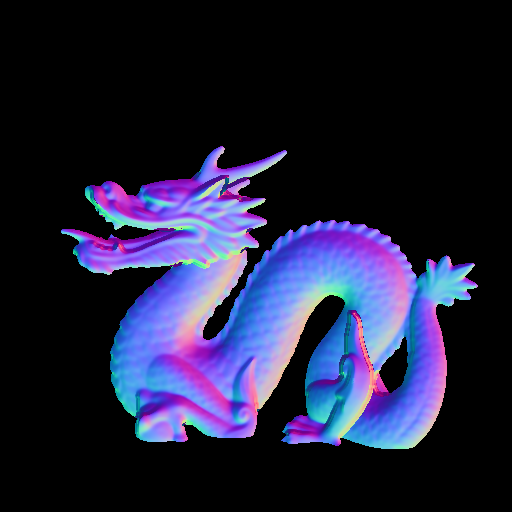
\includegraphics[width=.25\textwidth]{./Figures/svd-synthetic/no-noise/fancy_eval_2_normal_SVD.png}
	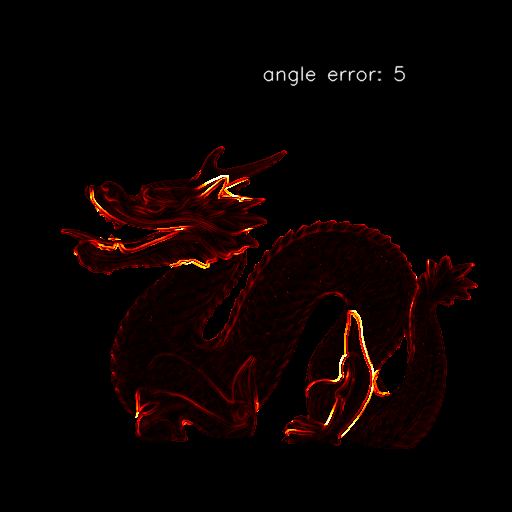
\includegraphics[width=.25\textwidth]{./Figures/svd-synthetic/no-noise/fancy_eval_2_error_SVD.png}
	\decoRule
	\label{fig:svd-normal}
	\caption{Normal map of a dragon object predicted by neighbor based method. k=2, angle error=5 \textbf{Left}: ground-truth normal map \textbf{Middle}: predicted normal map, \textbf{Right}: Error map}
\end{figure}
The neighbor based method is depended on a well-chosen parameter $ k $. Figure \ref{fig:svd-k-eval} shows the evaluation on different $ k $ values. When $ k=1 $, the average error of the whole image is the lowest one, most of the normals are close to the ground-truth but the outline edges, which are the areas that surface normal changed extremely sever. For the case $ k=2 $, the sharp edges are more smooth and cause more error, like the eyes area of the dragon. Compare to the first case, the outline edge error goes better. Most of the edge errors are reduced when $ k=2 $, since more neighbor points join the evaluation and it reduces the effect of outliers. However, for the area of horn outline, hindleg outline, the error goes worse. In this case, most of the neighbors of these points are outliers and thus failed this approach.  $ k=3 $ and $ k=4 $ further increase the angle errors based on $ k=2 $.
\begin{figure}[th]
	\centering
	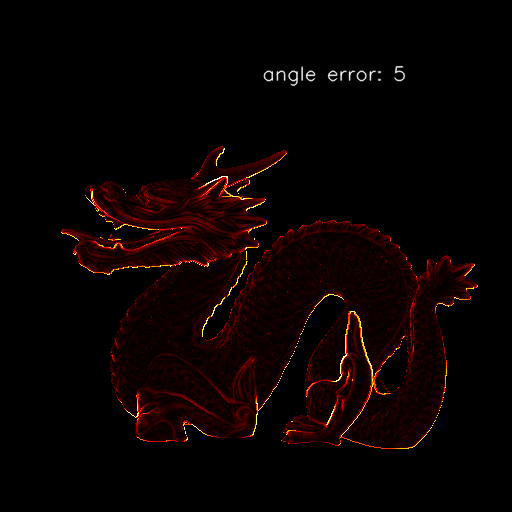
\includegraphics[width=.2\textwidth]{./Figures/svd-synthetic/k-compare/k1.png}
	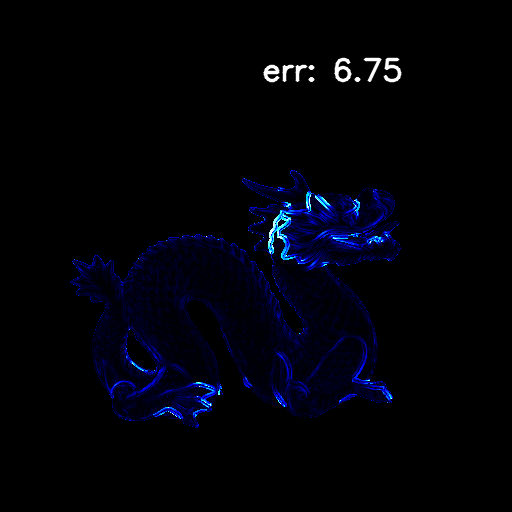
\includegraphics[width=.2\textwidth]{./Figures/svd-synthetic/k-compare/k2.png}
	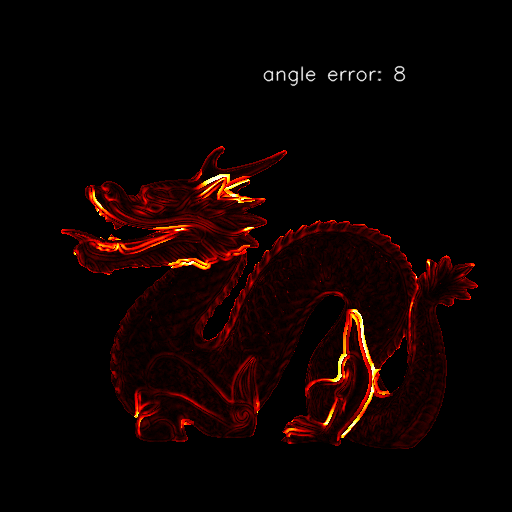
\includegraphics[width=.2\textwidth]{./Figures/svd-synthetic/k-compare/k3.png}
	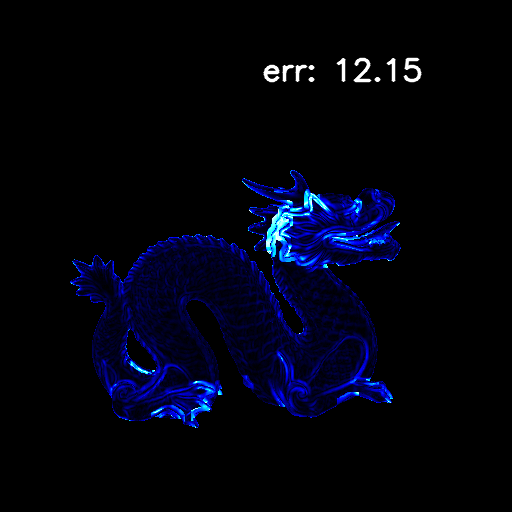
\includegraphics[width=.2\textwidth]{./Figures/svd-synthetic/k-compare/k4.png}	
	\decoRule
	\label{fig:svd-k-eval}
	\caption{Error map of neighbor based method with different $ k $ values. From left to right, $ k=1,2,3,4 $ separately.}
\end{figure}

The performance of neighbor based method is good enough for a well chosen $ k $. However, for the case of noised point cloud as input, this approach will broken, since the noise will failed the neighbor assumption and also reduce the number of possible neighbors of each point for a fixed $ k $.
\begin{figure}[th]
	\centering
	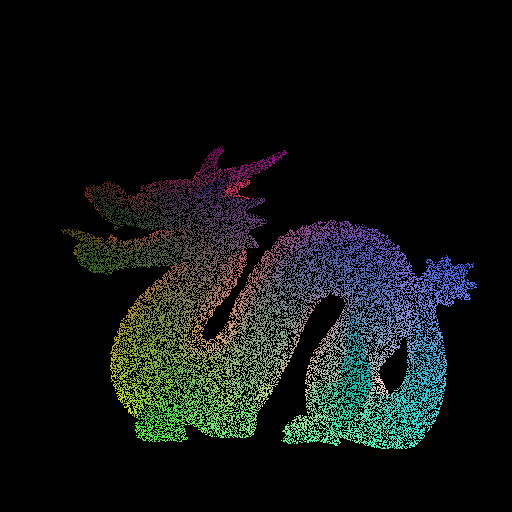
\includegraphics[width=.2\textwidth]{./Figures/svd-synthetic/noise/fancy_eval_2_point_cloud_noise.png}
	\includegraphics[width=.2\textwidth]{./Figures/svd-synthetic/noise/fancy_eval_2_groundtruth.png}
	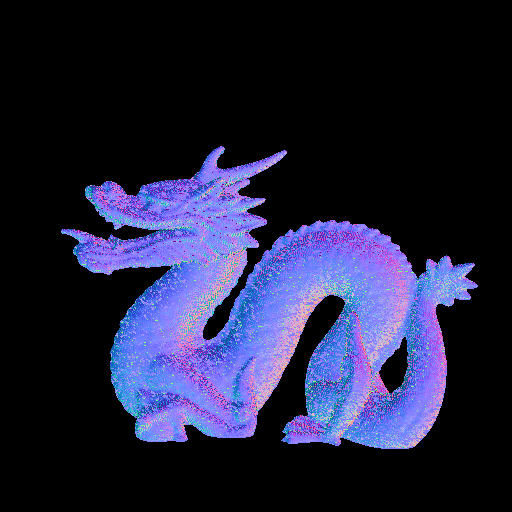
\includegraphics[width=.2\textwidth]{./Figures/svd-synthetic/noise/fancy_eval_2_normal_SVD.png}
	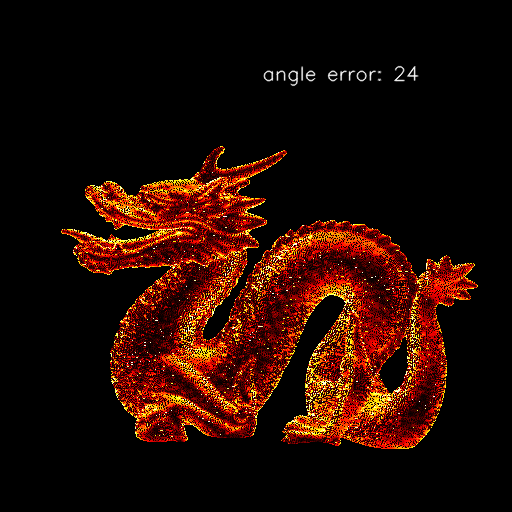
\includegraphics[width=.2\textwidth]{./Figures/svd-synthetic/noise/fancy_eval_2_error_SVD.png}	
	\decoRule
	\label{fig:svd-noise}
	\caption{SVD visual evaluation on a noised dragon model ($ 128\times128 $)}
\end{figure}

\section{Visual evaluation on GCNN model}
A qualitative evaluation on object "dragon" is shown in Figure \ref{fig:gcnn-eval}. As shown in the figure, GCNN model achieved a mean angle error in 9 degrees on this dragon object. The image has an overall good performance on the whole object. A closer evaluation is shown in Figure \ref{fig:gcnn-eval-synthetic-zoom-in}, the normal accuracy especially good on the smooth surface, like the body area. In the same case, NOC model as shown in Figure. \ref{fig:gcnn-eval-multi-model} has a overall worse normal than GCNN model in the smooth area. CNN model keeps the skip connection thus gives a sharper result than NOC model, however, the overall smooth part of the model is still worse than GCNN. Besides, the sharp area like the hindleg and the head area of dragon object, CNN model gives a much brighter error map (which means a higher angle error).

Figure \ref{fig:gcnn-eval-more} shows more evaluation on GCNN model. Although we can get a good result from GCNN model but from model ``Washington" we still can see it lacks the sharpness in the detail area like the face and clothes area. 


%% GCNN-eval
\begin{figure}[H]
	\centering
	\begin{subfigure}[b]{0.24\linewidth}
		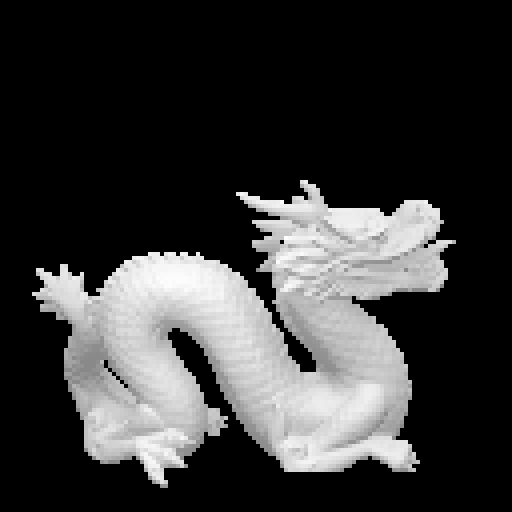
\includegraphics[width=\linewidth]{./Figures/gcnn_synthetic/fancy_eval_7_img.png}
		\caption{Image}
	\end{subfigure}
	\begin{subfigure}[b]{0.24\linewidth}
		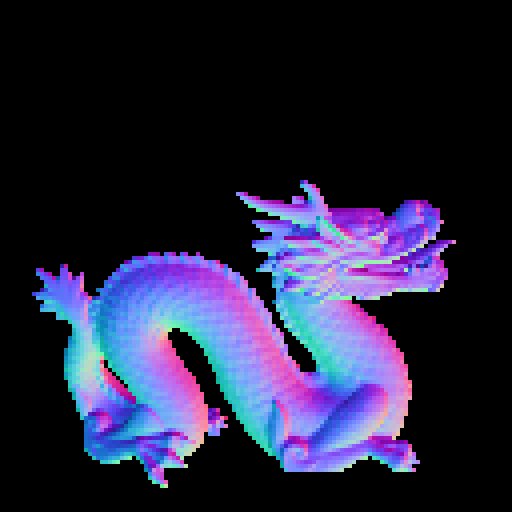
\includegraphics[width=\linewidth]{./Figures/gcnn_synthetic/fancy_eval_7_groundtruth.png}
		\caption{GT}
	\end{subfigure}
	\begin{subfigure}[b]{0.24\linewidth}
		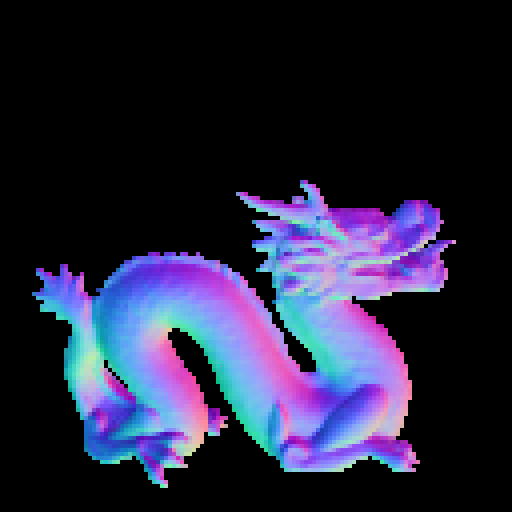
\includegraphics[width=\linewidth]{./Figures/gcnn_synthetic/fancy_eval_7_normal_GCNN-GCNN.png}
		\caption{Predict}
	\end{subfigure}
	\begin{subfigure}[b]{0.24\linewidth}
		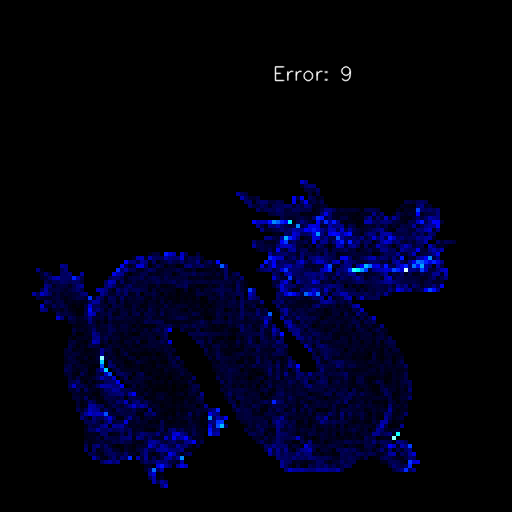
\includegraphics[width=\linewidth]{./Figures/gcnn_synthetic/fancy_eval_7_error_GCNN-GCNN.png}
		\caption{Error}
	\end{subfigure}
	
	\begin{tikzpicture}
		\node[text width=0.1\textwidth] at (11,-1) {90};
		\node[inner sep=0pt] (input) at (8,-1)
		{
\includegraphics[width=.2\textwidth]{./Figures/colorscale_blue.png}};
		\node[text width=0.3\textwidth] at (7,-1) {Error: 0};
	\end{tikzpicture}
	\decoRule
	\caption{GCNN visual evaluation. Window size $ 128\times128 $}
	\label{fig:gcnn-eval}
\end{figure}

%% GCNN zoom in eval
\begin{figure}[th]
	\centering
	\begin{subfigure}[b]{0.18\linewidth}
		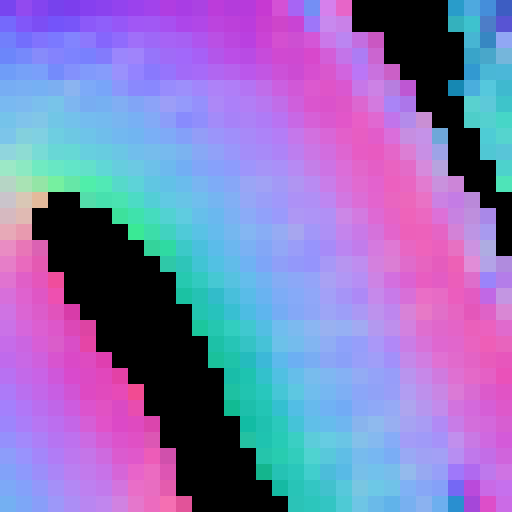
\includegraphics[width=\linewidth]{./Figures/gcnn_synthetic/eval_7_22_-8_normal.png}
	\end{subfigure}
	\begin{subfigure}[b]{0.18\linewidth}
		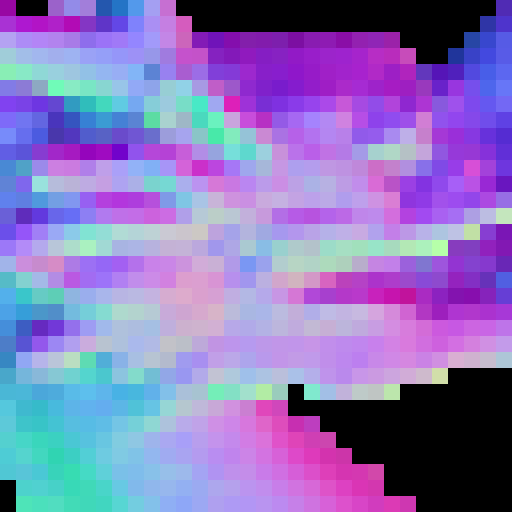
\includegraphics[width=\linewidth]{./Figures/gcnn_synthetic/eval_7_2_22_normal.png}
	\end{subfigure}
	\begin{subfigure}[b]{0.18\linewidth}
		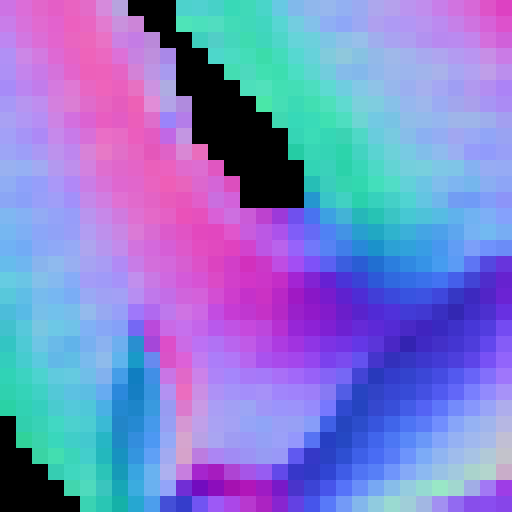
\includegraphics[width=\linewidth]{./Figures/gcnn_synthetic/eval_7_32_12_normal.png}
	\end{subfigure}
	\begin{subfigure}[b]{0.18\linewidth}
		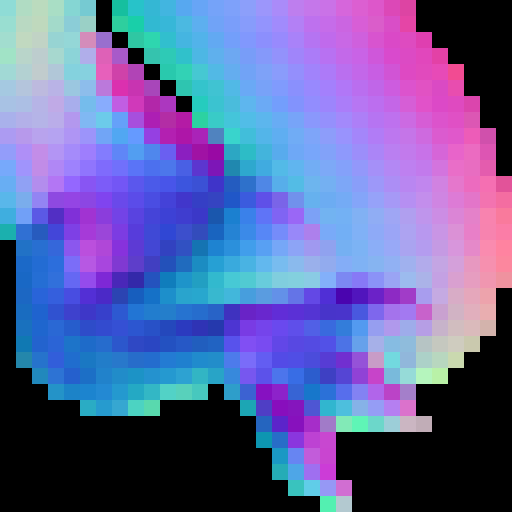
\includegraphics[width=\linewidth]{./Figures/gcnn_synthetic/eval_7_42_-28_normal.png}
	\end{subfigure}
	\begin{subfigure}[b]{0.18\linewidth}
		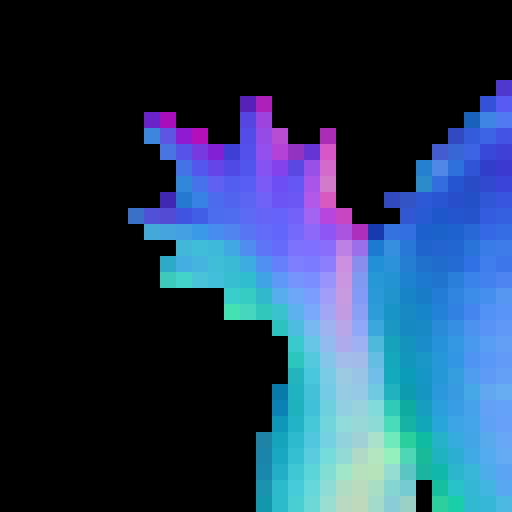
\includegraphics[width=\linewidth]{./Figures/gcnn_synthetic/eval_7_12_-48_normal.png}
	\end{subfigure}
	
	\begin{subfigure}[b]{0.18\linewidth}
		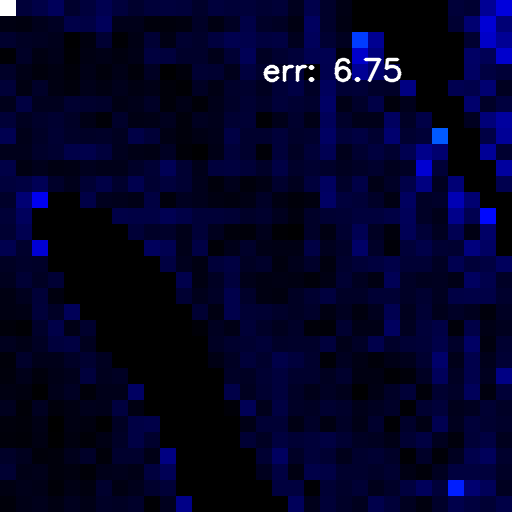
\includegraphics[width=\linewidth]{./Figures/gcnn_synthetic/eval_7_22_-8_error.png}
		\caption{Scale}
	\end{subfigure}
	\begin{subfigure}[b]{0.18\linewidth}
		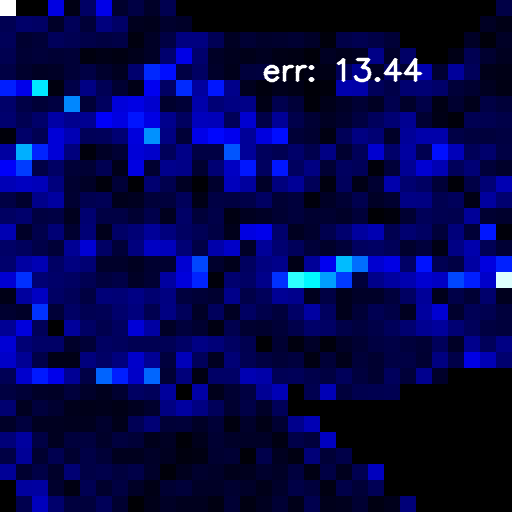
\includegraphics[width=\linewidth]{./Figures/gcnn_synthetic/eval_7_2_22_error.png}
		\caption{Head}
	\end{subfigure}
	\begin{subfigure}[b]{0.18\linewidth}
		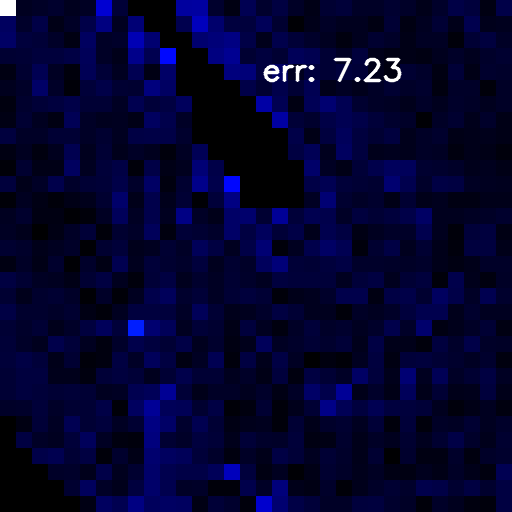
\includegraphics[width=\linewidth]{./Figures/gcnn_synthetic/eval_7_32_12_error.png}
		\caption{Foreleg}
	\end{subfigure}
	\begin{subfigure}[b]{0.18\linewidth}
		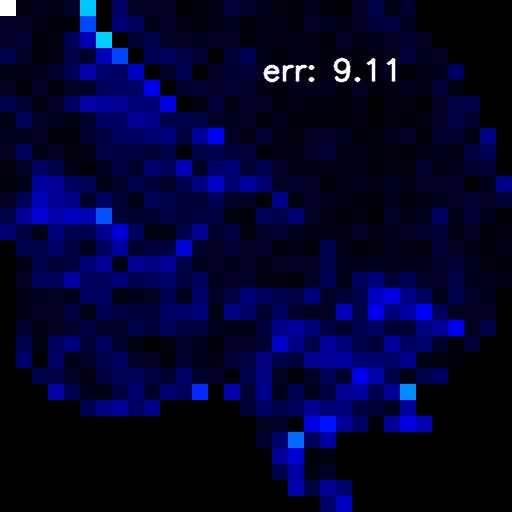
\includegraphics[width=\linewidth]{./Figures/gcnn_synthetic/eval_7_42_-28_error.png}
		\caption{Hindleg}
	\end{subfigure}
	\begin{subfigure}[b]{0.18\linewidth}
		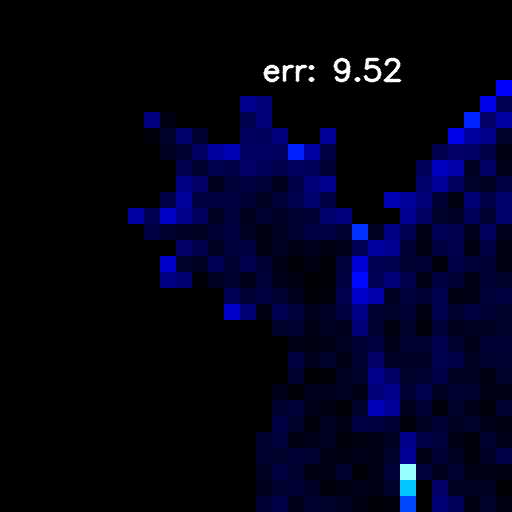
\includegraphics[width=\linewidth]{./Figures/gcnn_synthetic/eval_7_12_-48_error.png}
		\caption{Tail}
	\end{subfigure}
	
	\decoRule
	\caption{Zoom in of some regions of Dragon object (GCNN models). Window size $ 32\times32 $.}
	\label{fig:gcnn-eval-synthetic-zoom-in}
\end{figure}

%% compare to other models

%% GCNN zoom in eval
\begin{figure}[H]
	\centering
	\begin{subfigure}[b]{0.24\linewidth}
		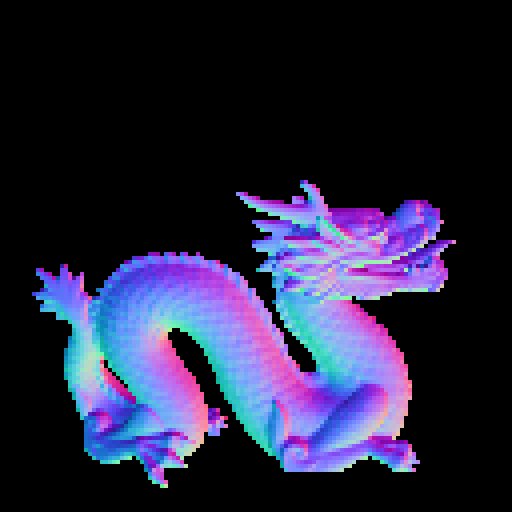
\includegraphics[width=\linewidth]{./Figures/gcnn_synthetic/fancy_eval_7_groundtruth.png}
	\end{subfigure}
	\begin{subfigure}[b]{0.24\linewidth}
		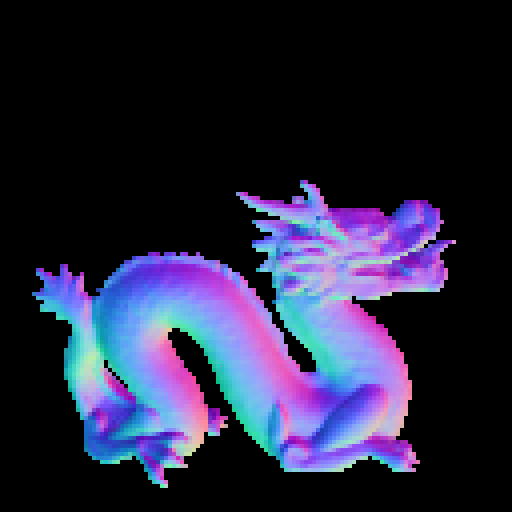
\includegraphics[width=\linewidth]{./Figures/gcnn_synthetic/fancy_eval_7_normal_GCNN-GCNN.png}
	\end{subfigure}
	\begin{subfigure}[b]{0.24\linewidth}
		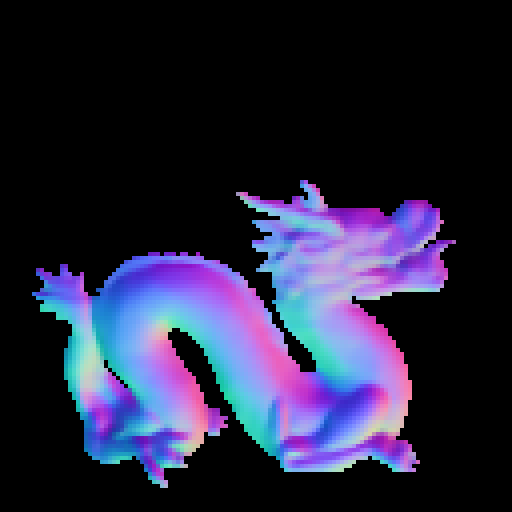
\includegraphics[width=\linewidth]{./Figures/gcnn_synthetic/fancy_eval_7_normal_GCNN-NOC.png}
	\end{subfigure}
	\begin{subfigure}[b]{0.24\linewidth}
		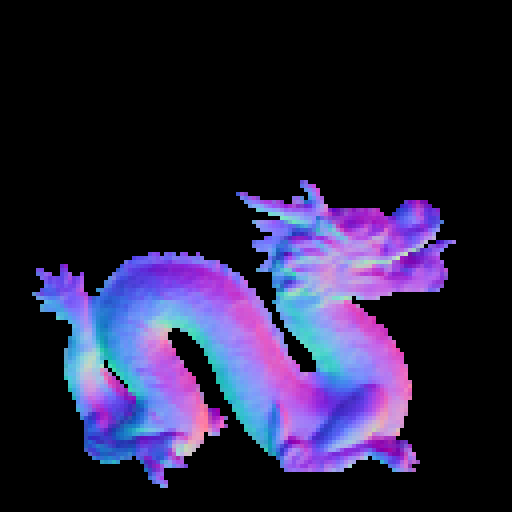
\includegraphics[width=\linewidth]{./Figures/gcnn_synthetic/fancy_eval_7_normal_GCNN-CNN.png}
	\end{subfigure}
	
	\begin{subfigure}[b]{0.24\linewidth}
		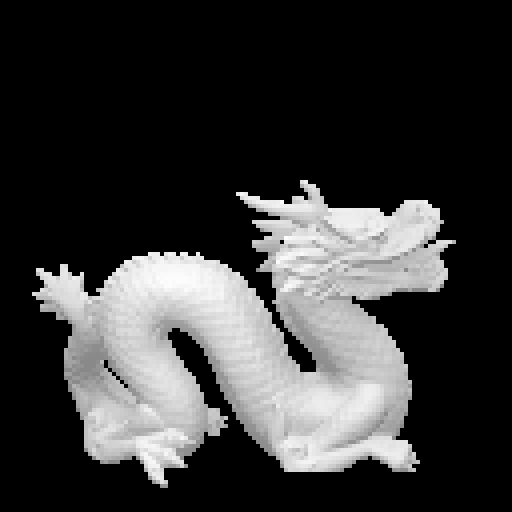
\includegraphics[width=\linewidth]{./Figures/gcnn_synthetic/fancy_eval_7_img.png}
		\caption{GT}
	\end{subfigure}
	\begin{subfigure}[b]{0.24\linewidth}
		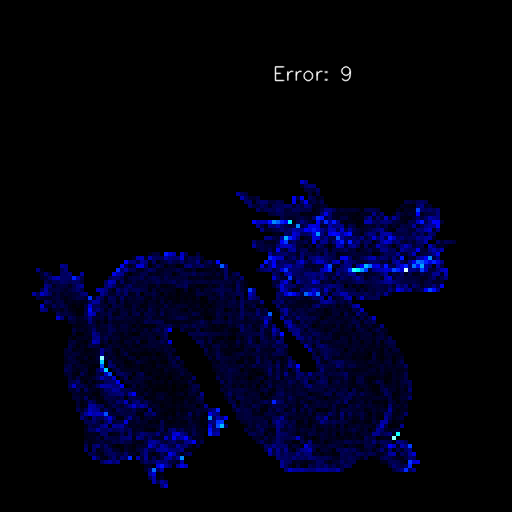
\includegraphics[width=\linewidth]{./Figures/gcnn_synthetic/fancy_eval_7_error_GCNN-GCNN.png}
		\caption{GCNN}
	\end{subfigure}
	\begin{subfigure}[b]{0.24\linewidth}
		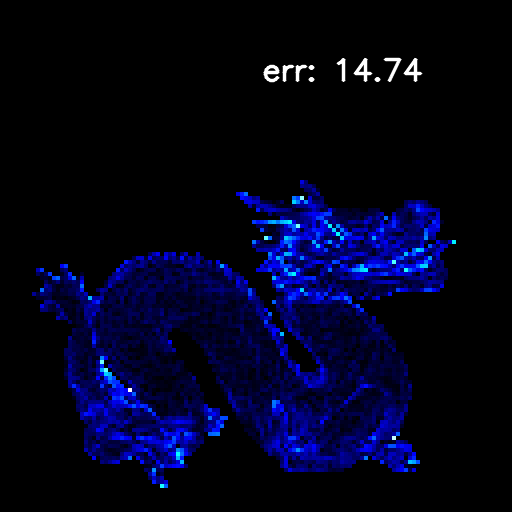
\includegraphics[width=\linewidth]{./Figures/gcnn_synthetic/fancy_eval_7_error_GCNN-NOC.png}
		\caption{NOC}
	\end{subfigure}
	\begin{subfigure}[b]{0.24\linewidth}
		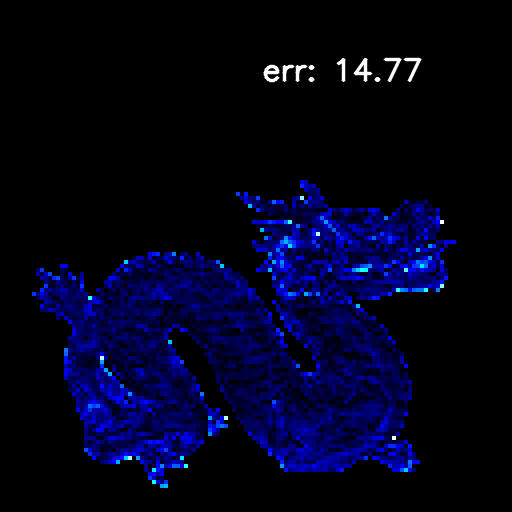
\includegraphics[width=\linewidth]{./Figures/gcnn_synthetic/fancy_eval_7_error_GCNN-CNN.png}
		\caption{CNN}
	\end{subfigure}
	
	\decoRule
	\caption{Comparison of GCNN based models.}
	\label{fig:gcnn-eval-multi-model}
\end{figure}


\section{ Discussion about the feature maps of GCNN architecture models}

As shown in figure \ref{fig:gcnn-cnn-feature map}, we also visualize the feature maps of the last gated convolution layer in the first up-sampling part for CNN and GCNN models, which corresponding the feature maps with size $ 32\times 32 $ in width and height. The input data is also same dragon object that we used for normal visualization. For each feature map, we map the minimum value to the left-most color in the color bar and the maximum value to the right-most color in the color bar. 
We want to discuss the the different of the feature maps between CNN, NOC and GCNN models.

In order to see the result clearly, we use one color for the feature map visualization and use the brightness to distinguish the scale of the vales, the white corresponds 1, the black corresponds 0, green color corresponds some value in between. 

From the CNN feature maps, we can see that the brightness areas are distributed all around the feature maps. For the GCNN feature maps, the brightness areas are usually concentrate only in few pixels. If we map the brightness areas to the original image, they correspond to the dense sharp edges areas, which is usually the hardest areas for normal estimation task. We suspect that these feature maps are the detail feature maps that extract from sharp edges. Based on this assumption, we can say that gated convolution layer describes the detail features in a more accurate way compare to standard convolution layer, since the brightness areas is smaller. Most of the GCNN feature maps usually has only one bright pixel with a few set of dim green pixels whereas CNN feature maps has more bright pixels with a lot of dim pixels all around the image. This accurate feature extraction provides our GCNN model a better performance on the detail area.

Second, for the GCNN model,  we observed that some feature maps have no  small bright areas but bright areas distributed evenly on the whole object. Some of the feature maps has a overall medium value some has a value close to 1. Nevertheless, these feature maps are different from the detail feature maps with only few pixels with high values(brightness). We suspect that these features maps provides an over-view of the objects for a coarse prediction. So that they can cooperate with detail feature maps to sharpen the prediction. It also holds for NOC model, since it does not equip with skip connection, most of the feature maps are global feature maps with an evenly bright feature maps, so that the corresponding normal maps predicted by NOC model are more coarse. For the CNN model, there also exists global feature maps, however, they are mostly incomplete, either missing the tails or missing the paws. 
Actually, these missing areas can usually be found in the detail feature maps. This also explained why the CNN detail feature maps has too much brightness areas, the detail feature maps and global feature maps are mixed together. And this unclear feature map extractor leads to the weak performance on normal estimation.

%% feature maps comparison
\begin{figure}[H]
	\centering
	
	\begin{subfigure}[b]{\linewidth}
		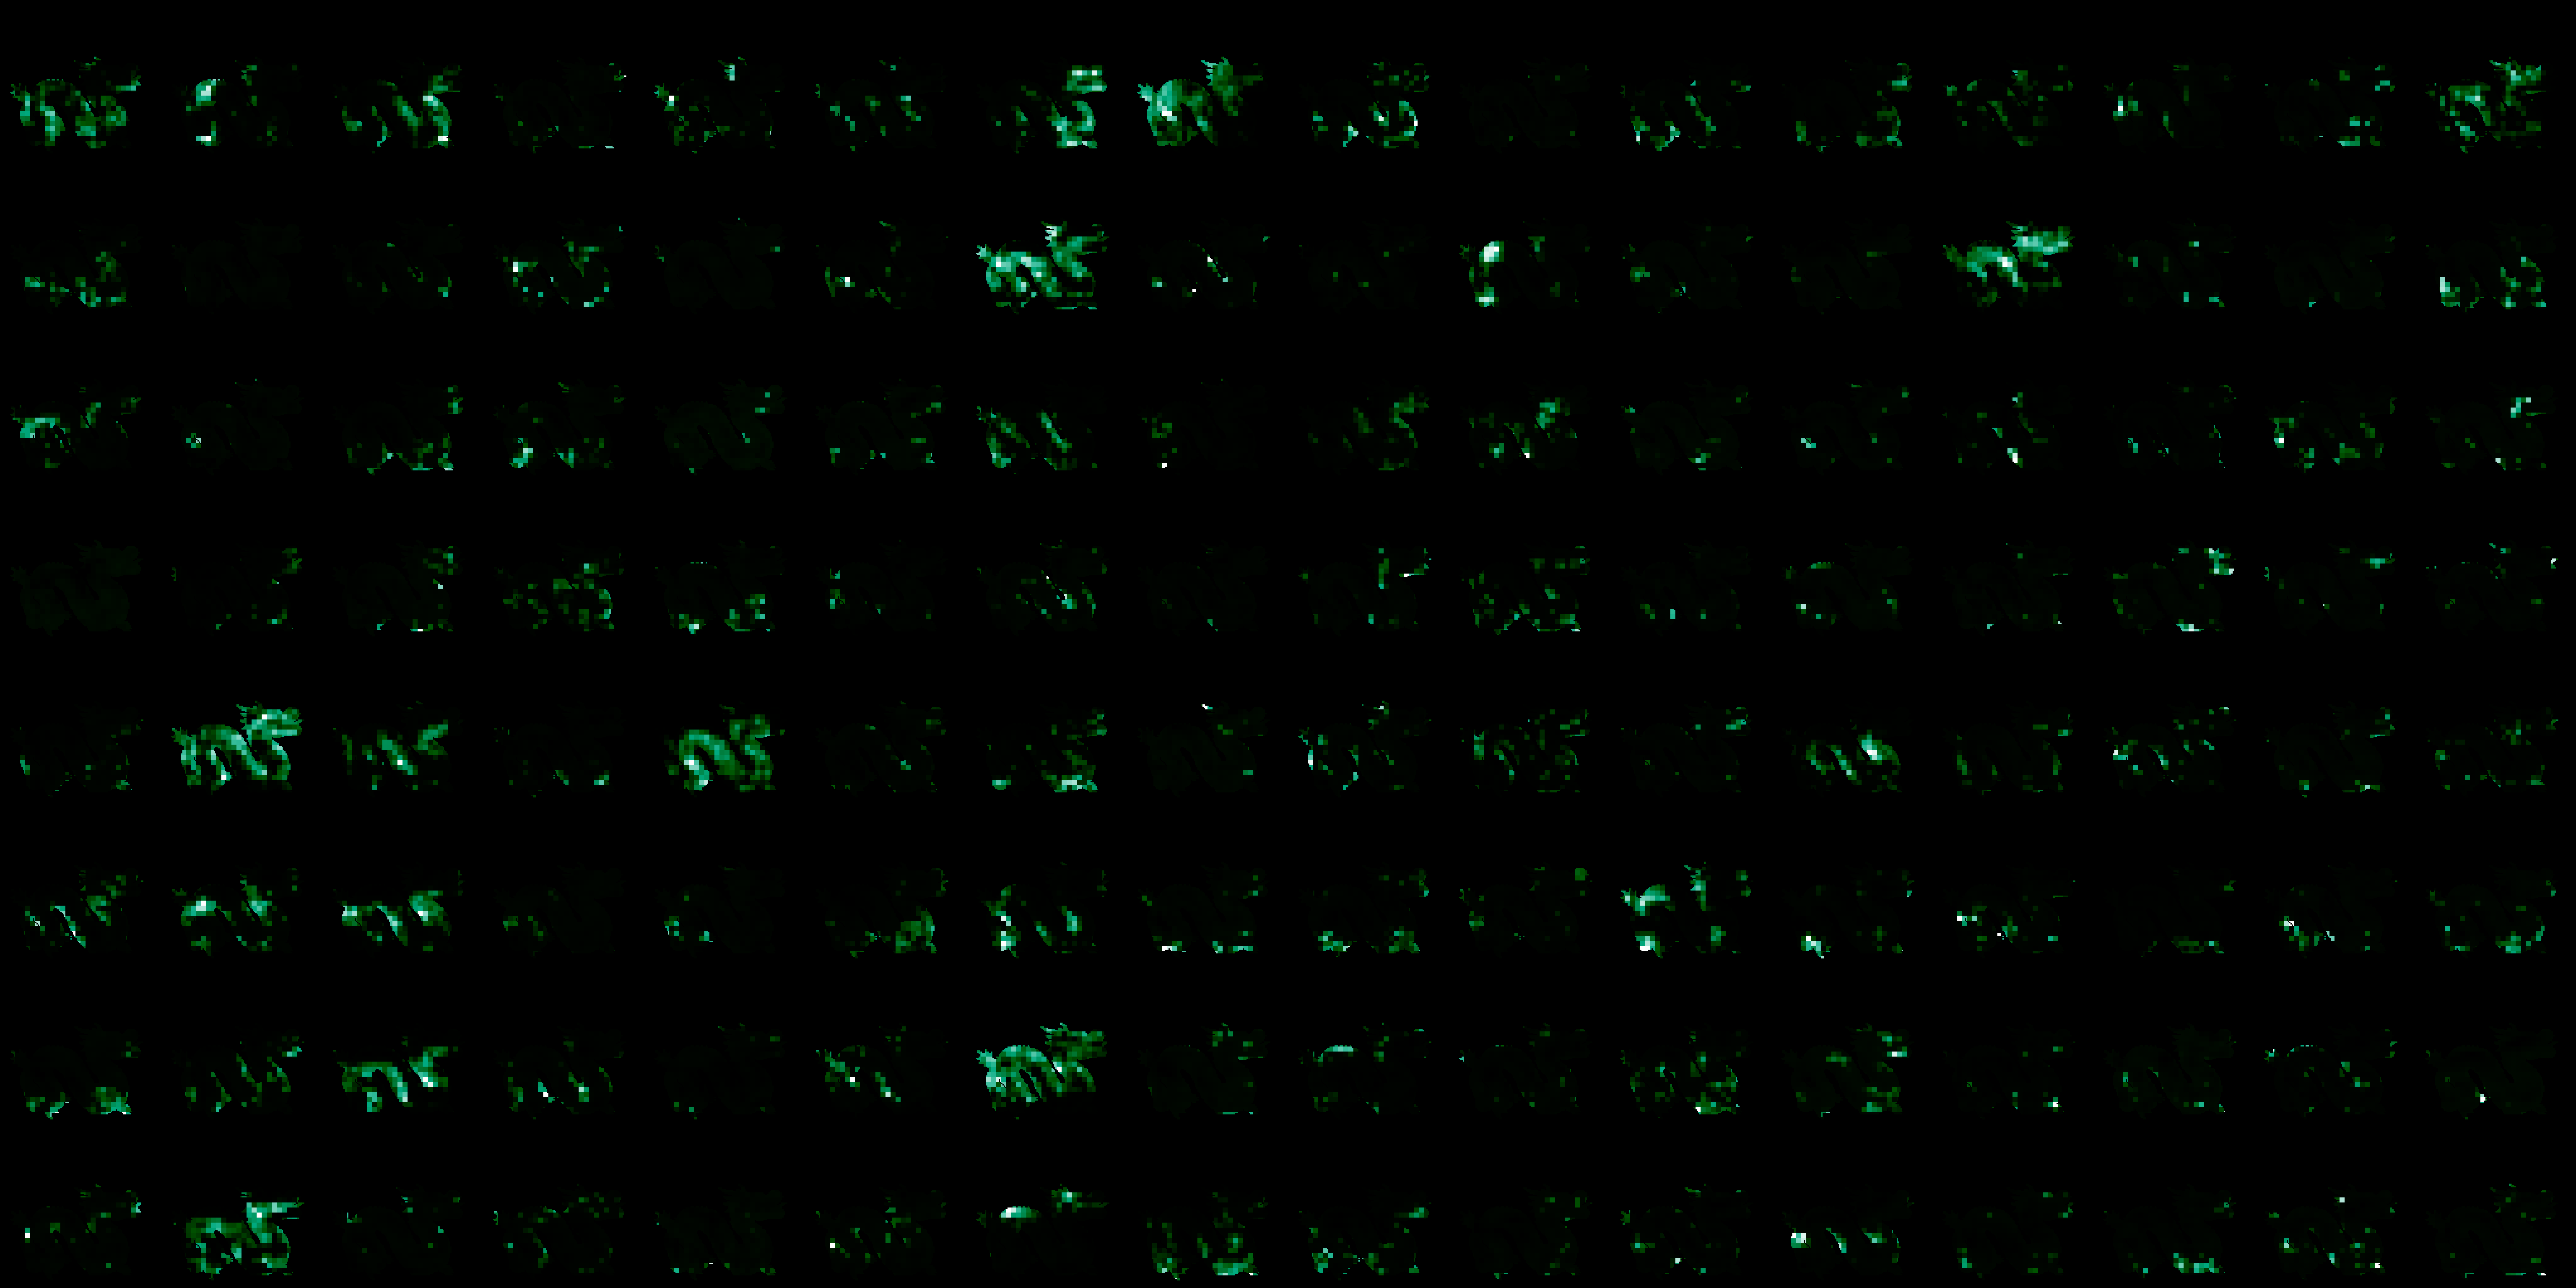
\includegraphics[width=\linewidth]{./Figures/feature_map_gcnn/feature_map_gcnn-cnn.png}
		\caption{CNN Feature Maps}
	\end{subfigure}
	
	\begin{subfigure}[b]{\linewidth}
		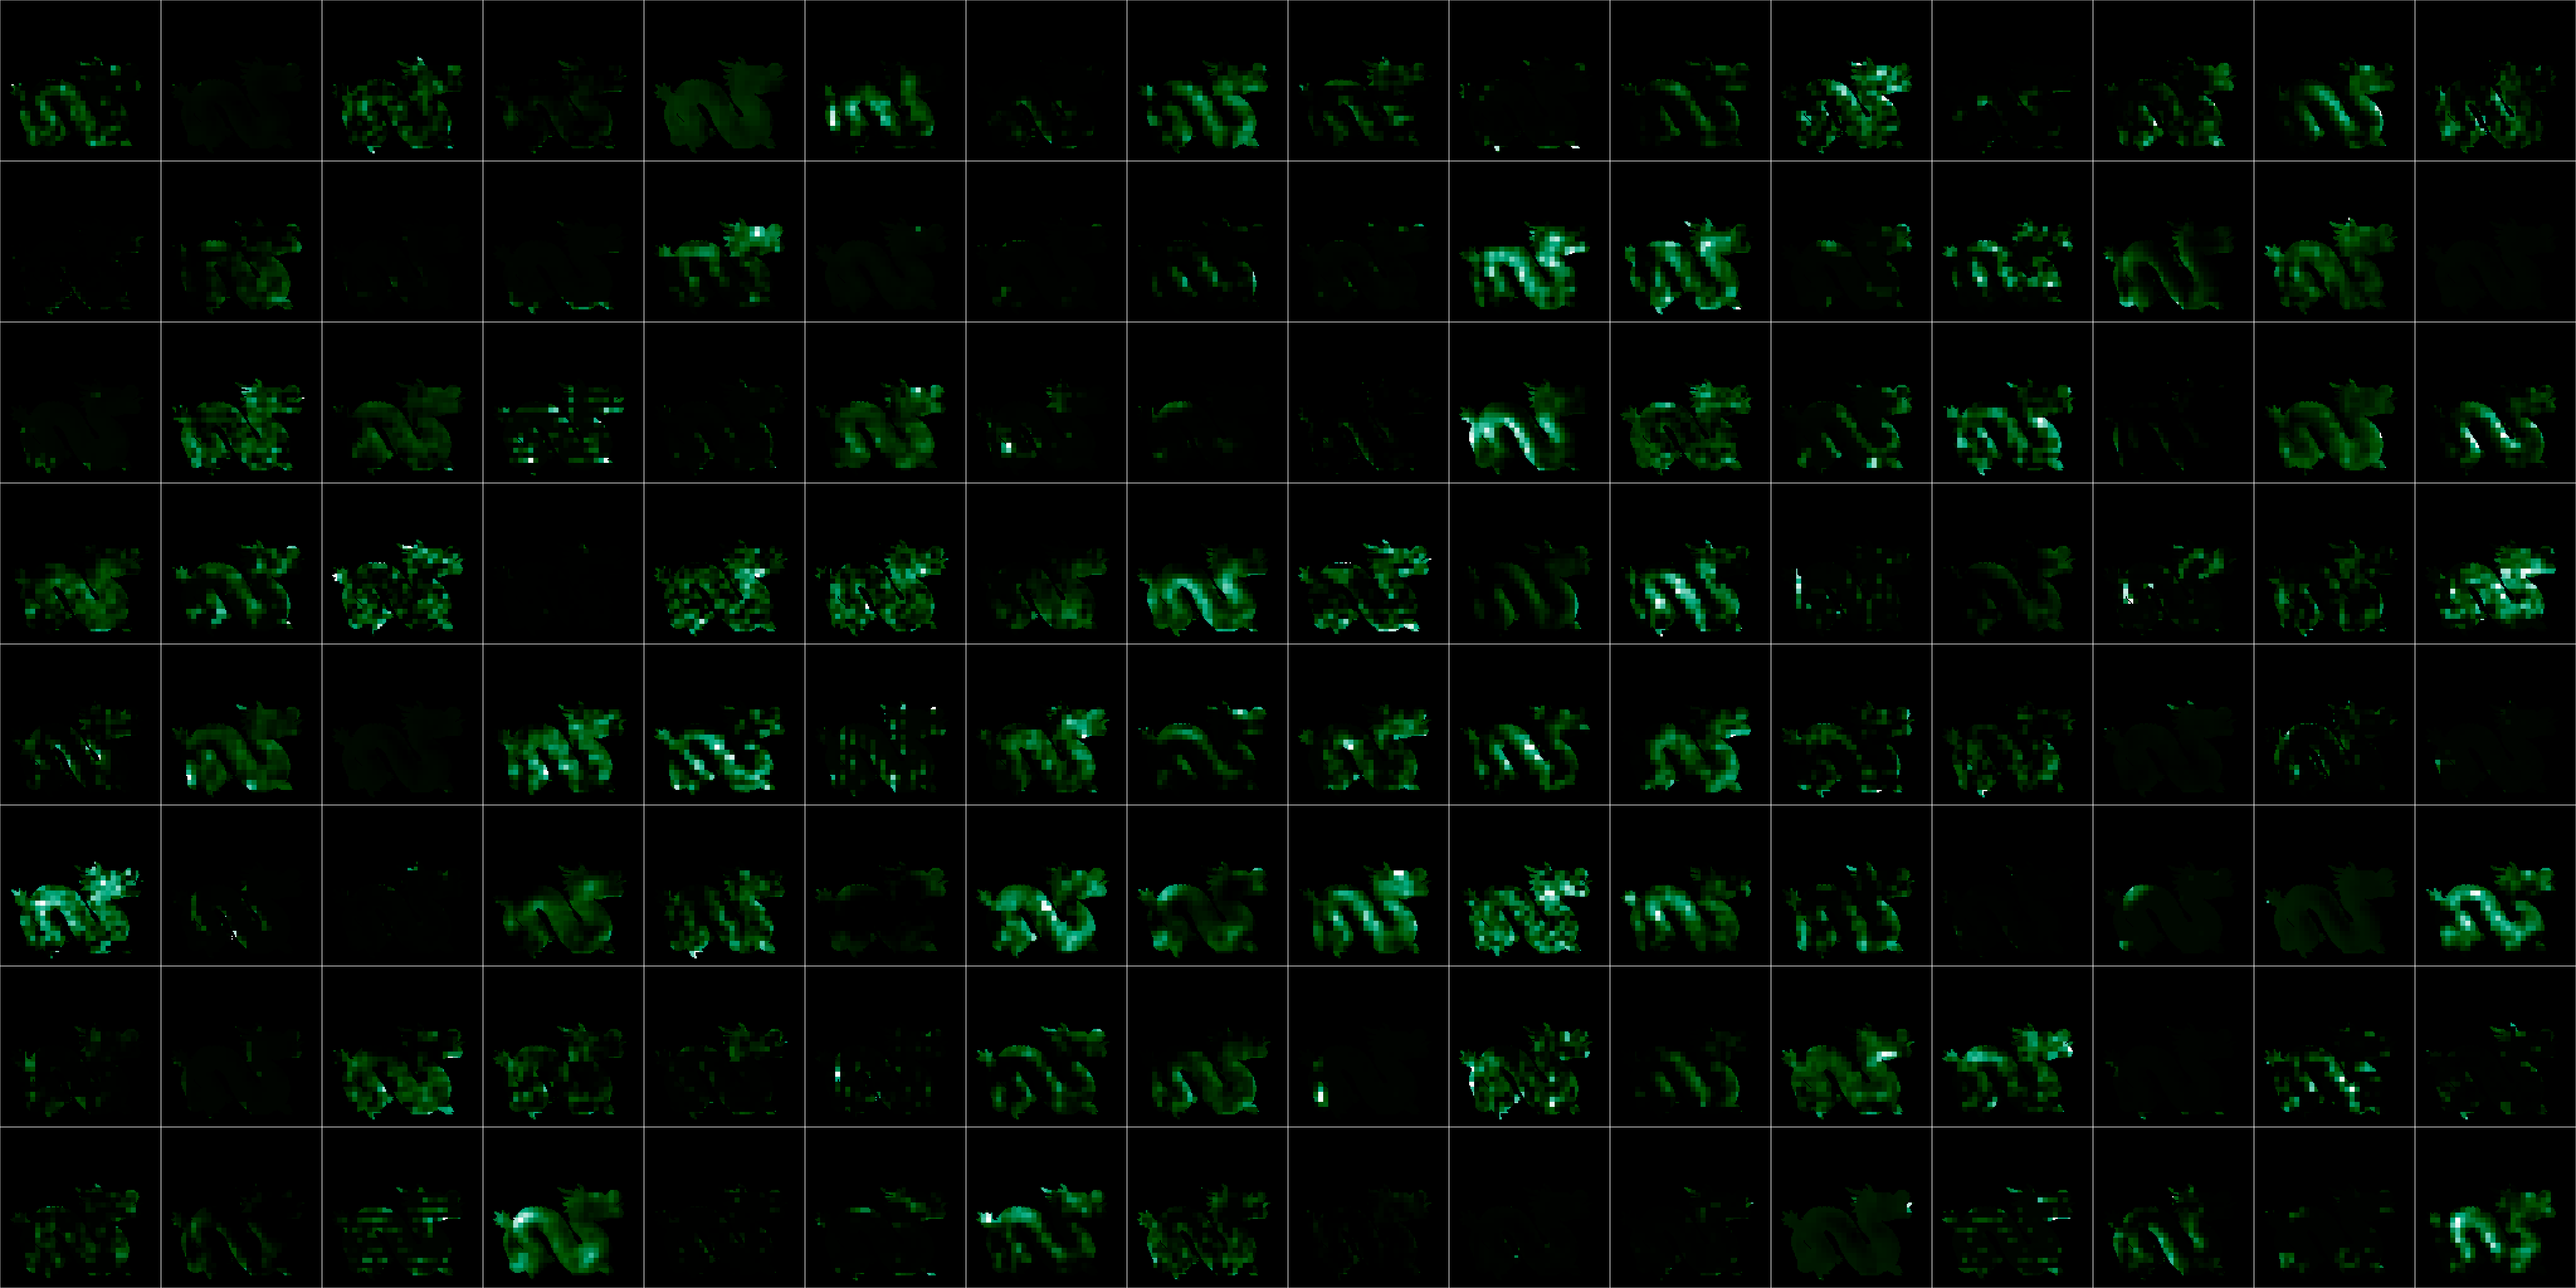
\includegraphics[width=\linewidth]{./Figures/feature_map_gcnn/feature_map_gcnn-noc.png}
		\caption{NOC Feature Maps}
	\end{subfigure}

	\begin{subfigure}[b]{\linewidth}
	\includegraphics[width=\linewidth]{./Figures/feature_map_gcnn/feature_map_gcnn-gcnn.png}
	\caption{GCNN Feature Maps}
\end{subfigure}
	
		\begin{tikzpicture}
		\node[text width=0.1\textwidth] at (11,-1) {90};
		\node[inner sep=0pt] (input) at (8,-1)
		{
\includegraphics[width=.2\textwidth]{./Figures/colorscale_deepgreen.jpg}};
		\node[text width=0.3\textwidth] at (7,-1) {Error: 0};
	\end{tikzpicture}
	\decoRule
	\caption{Feature maps of GCNN architecture based models at the first up-sampling gated convolution layer. All 128 feature maps are visualized for each model with normalization and filtered background.}
	\label{fig:gcnn-cnn-feature map}
\end{figure}


\newpage 
\section{Visual evaluation on Trip-Net models }

For the approach using illuminated calibrated RGBD image, the task is undertaken by Trip-Net introduced in \ref{sec:trip-net}. The Trip-Net uses illuminated information align with the geometry information achieves a sharper and more accurate result compare to the GCNN model.

%% TripNet-eval
\begin{figure}[H]
	\centering
	\begin{subfigure}[b]{0.24\linewidth}
		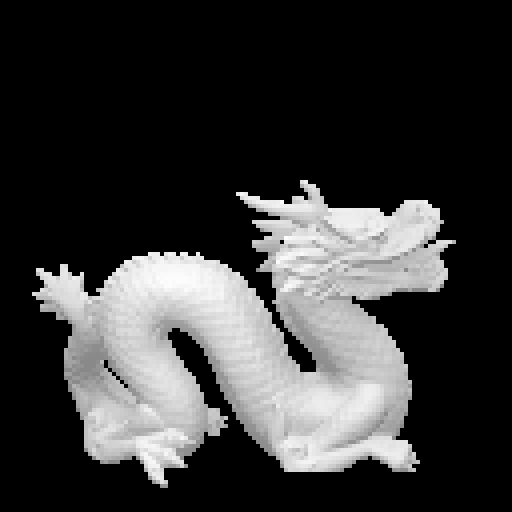
\includegraphics[width=\linewidth]{./Figures/gcnn_synthetic/fancy_eval_7_img.png}
		\caption{Image}
	\end{subfigure}
	\begin{subfigure}[b]{0.24\linewidth}
		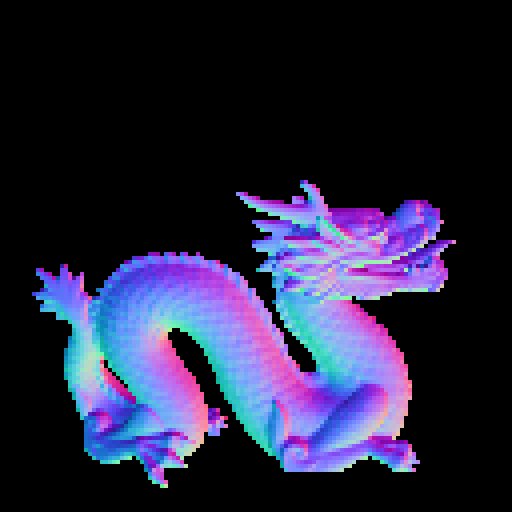
\includegraphics[width=\linewidth]{./Figures/gcnn_synthetic/fancy_eval_7_groundtruth.png}
		\caption{GT}
	\end{subfigure}
	\begin{subfigure}[b]{0.24\linewidth}
		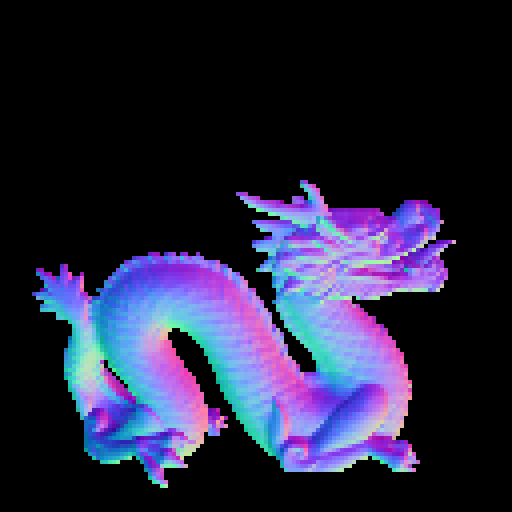
\includegraphics[width=\linewidth]{./Figures/gcnn_synthetic/fancy_eval_7_normal_an2-8-1000.png}
		\caption{Predict}
	\end{subfigure}
	\begin{subfigure}[b]{0.24\linewidth}
		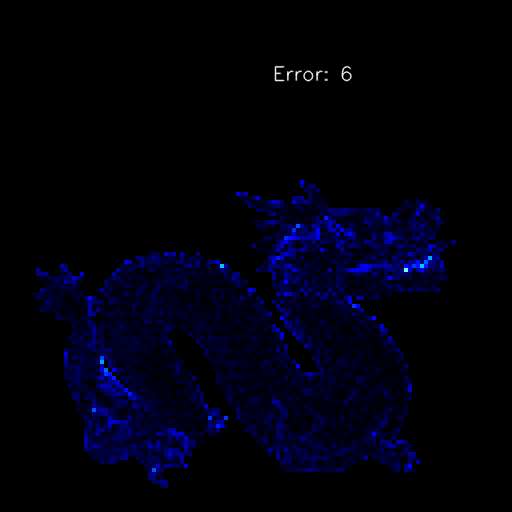
\includegraphics[width=\linewidth]{./Figures/gcnn_synthetic/fancy_eval_7_error_an2-8-1000.png}
		\caption{Error}
	\end{subfigure}
	
	\begin{tikzpicture}
		\node[text width=0.1\textwidth] at (11,-1) {90};
		\node[inner sep=0pt] (input) at (8,-1)
		{\includegraphics[width=.2\textwidth]{./Figures/colorscale_blue.png}};
		\node[text width=0.3\textwidth] at (7,-1) {Error: 0};
	\end{tikzpicture}
	\decoRule
	\caption{Trip-Net visual evaluation on resolution $ 128\times128 $}
	\label{fig:trip-eval}
\end{figure}



The qualitative evaluation is shown in figure \ref{fig:trip-eval}. In order to show the effectiveness of added illuminated information, the training settings for all the models are exact the same. We also use the same input as we did in GCNN evaluation. The error of Trip-Net is 6 degree whereas the GCNN is 9. 


%% tripNet zoom in eval
\begin{figure}[H]
	\centering
	\begin{subfigure}[b]{0.18\linewidth}
		\includegraphics[width=\linewidth]{./Figures/trip_net_zoom_in/eval_7_22_-8_normal.png}
	\end{subfigure}
	\begin{subfigure}[b]{0.18\linewidth}
		\includegraphics[width=\linewidth]{./Figures/trip_net_zoom_in/eval_7_2_22_normal.png}
	\end{subfigure}
	\begin{subfigure}[b]{0.18\linewidth}
		\includegraphics[width=\linewidth]{./Figures/trip_net_zoom_in/eval_7_32_12_normal.png}
	\end{subfigure}
	\begin{subfigure}[b]{0.18\linewidth}
		\includegraphics[width=\linewidth]{./Figures/trip_net_zoom_in/eval_7_42_-28_normal.png}
	\end{subfigure}
	\begin{subfigure}[b]{0.18\linewidth}
		\includegraphics[width=\linewidth]{./Figures/trip_net_zoom_in/eval_7_12_-48_normal.png}
	\end{subfigure}
	
	\begin{subfigure}[b]{0.18\linewidth}
		\includegraphics[width=\linewidth]{./Figures/trip_net_zoom_in/eval_7_22_-8_error.png}
		\caption{Scale}
	\end{subfigure}
	\begin{subfigure}[b]{0.18\linewidth}
		\includegraphics[width=\linewidth]{./Figures/trip_net_zoom_in/eval_7_2_22_error.png}
		\caption{Head}
	\end{subfigure}
	\begin{subfigure}[b]{0.18\linewidth}
		\includegraphics[width=\linewidth]{./Figures/trip_net_zoom_in/eval_7_32_12_error.png}
		\caption{Foreleg}
	\end{subfigure}
	\begin{subfigure}[b]{0.18\linewidth}
		\includegraphics[width=\linewidth]{./Figures/trip_net_zoom_in/eval_7_42_-28_error.png}
		\caption{Hindleg}
	\end{subfigure}
	\begin{subfigure}[b]{0.18\linewidth}
		\includegraphics[width=\linewidth]{./Figures/trip_net_zoom_in/eval_7_12_-48_error.png}
		\caption{Tail}
	\end{subfigure}
	
	\decoRule
	\caption{Zoom in of detail regions ( $ 32\times32 $ ) of Dragon object (Trip-Net model).}
	\label{fig:tripnet-eval-synthetic-zoom-in}
\end{figure}


As shown in the figure \ref{fig:tripnet-eval-synthetic-zoom-in}, the scale on the dragon body is much easier to detect and also close to the ground-truth. The head region gives a sharper edge prediction. All of the five sampled zoom-in regions in the Trip-Net has a better performance than GCNN. It seems that the illumination helps the model to learn sharper features in the network.





%% F1-F4 eval

\begin{figure}
	\centering
	\begin{subfigure}[b]{0.18\linewidth}
		\includegraphics[width=\linewidth]{./Figures/gcnn_synthetic/fancy_eval_7_groundtruth.png}
	\end{subfigure}
	\begin{subfigure}[b]{0.18\linewidth}
		\includegraphics[width=\linewidth]{./Figures/gcnn_synthetic/fancy_eval_7_normal_f1.png}
	\end{subfigure}
	\begin{subfigure}[b]{0.18\linewidth}
		\includegraphics[width=\linewidth]{./Figures/gcnn_synthetic/fancy_eval_7_normal_f2.png}
	\end{subfigure}
	\begin{subfigure}[b]{0.18\linewidth}
		\includegraphics[width=\linewidth]{./Figures/gcnn_synthetic/fancy_eval_7_normal_f3.png}
	\end{subfigure}
	\begin{subfigure}[b]{0.18\linewidth}
		\includegraphics[width=\linewidth]{./Figures/gcnn_synthetic/fancy_eval_7_normal_f4.png}
	\end{subfigure}
	
	
	\begin{subfigure}[b]{0.18\linewidth}
		\includegraphics[width=\linewidth]{./Figures/gcnn_synthetic/fancy_eval_7_img.png}
		\caption{GT}
	\end{subfigure}
	\begin{subfigure}[b]{0.18\linewidth}
		\includegraphics[width=\linewidth]{./Figures/gcnn_synthetic/fancy_eval_7_error_f1.png}
		\caption{F1}
	\end{subfigure}
	\begin{subfigure}[b]{0.18\linewidth}
		\includegraphics[width=\linewidth]{./Figures/gcnn_synthetic/fancy_eval_7_error_f2.png}
		\caption{F2}
	\end{subfigure}
	\begin{subfigure}[b]{0.18\linewidth}
		\includegraphics[width=\linewidth]{./Figures/gcnn_synthetic/fancy_eval_7_error_f3.png}
		\caption{F3}
	\end{subfigure}
	\begin{subfigure}[b]{0.18\linewidth}
		\includegraphics[width=\linewidth]{./Figures/gcnn_synthetic/fancy_eval_7_error_f4.png}
		\caption{F4}
	\end{subfigure}
	
	\decoRule
	\caption{Comparison between different fusion times on Trip-Net Architecture ($ 128\times128 $). }
	\label{fig:tripnet-eval-synthetic-zoom-in}
\end{figure}




\section{Trining on higher resolution}
We also prepared the dataset with resolution $ 512\times 512 $ for model evaluation. Higher resolution gives more information about the surface feature using the same model compare to lower resolution. The benefit is, if we extract a fixed sized patch from the normal map, say $ 32 \times 32 $, it might correspond a hindleg area of the dragon object in $ 128\times 128 $ resolution but maybe only a toe in $ 512\times 512 $ resolution. Therefore if we still use the same kernel size in the network for the same dataset, (like we did with $ 3\times 3 $) the higher the resolution it has, the less area it will cover. Thus the surface will more smooth and easy to calculate the surface normal. This is a good thing. Because then we might only need to use these $ 32\times 32 $ points to calculate a toe in $ 512\times512 $ resolution image. But in $ 128\times128 $ resolution image, the same area $ 32\times32 $ might corresponding to entire  hindleg of the dragon object. In another word, we can also say that the higher resolution ``smooth" the object surface. Thus the higher resolution helps the model to calculate a more accurate normal map. 


%% 5 degree metric
\begin{table}[H]
	\centering
	\begin{tabular}{l | l l l }
		\toprule
		\tabhead{Metrics} & \tabhead{SVD} & \tabhead{GCNN} & \tabhead{Trip-Net} \\
		\midrule
		Mean  					& 8.88 & 5.82 & 5.33 \\ 
		\hline
		Median					& 3.66 & 3.98 & 3.67 \\ 
		\hline
		$ 5^\circ $ 			& 0.63 & 0.63 & 0.66 \\
		\hline
		$ 11.5^\circ $ 			& 0.79 & 0.89 & 0.91 \\
		\hline
		$ 22.5^\circ $ 			& 0.89 & 0.97 & 0.97 \\
		\hline
		$ 30^\circ $ 			& 0.92 & 0.98 & 0.99 \\
		\bottomrule
	\end{tabular}
	\caption{High resolution dataset evaluation of SVD, GCNN and Trip-Net models on 6 different metrics based on 100 test scenes.}	
	\label{tab:high_resolution_eval}
\end{table}



Since our model is fully convolution network, the architecture keeps exactly same on the high resolution dataset. We use the same settings and the same models for training work on dataset with $ 512\times512 $ resolution. The training on high resolution network takes longer time but achieves a lower angle error. 




\newpage 
%% high resolution trip-net visualization
\begin{figure}[th]
	\centering
	\begin{subfigure}[b]{0.48\linewidth}
		\includegraphics[width=\linewidth]{./Figures/comparison_512/fancy_eval_11_normal_Trip-Net-512.png}
		\caption{Trip-Net}
	\end{subfigure}
	\begin{subfigure}[b]{0.48\linewidth}
		\includegraphics[width=\linewidth]{./Figures/comparison_512/fancy_eval_11_groundtruth.png}
		\caption{GT}
	\end{subfigure}
	
	
	\begin{subfigure}[b]{0.32\linewidth}
		\includegraphics[width=\linewidth]{./Figures/comparison_512/fancy_eval_11_point_cloud_noise.png}
		\caption{Input}
	\end{subfigure}
	\begin{subfigure}[b]{0.32\linewidth}
		\includegraphics[width=\linewidth]{./Figures/comparison_512/fancy_eval_11_img.png}
		\caption{Image}
	\end{subfigure}
	\begin{subfigure}[b]{0.32\linewidth}
		\includegraphics[width=\linewidth]{./Figures/comparison_512/fancy_eval_11_error_Trip-Net-512.png}
		\caption{Error}
	\end{subfigure}
	
	\begin{tikzpicture}
		\node[text width=0.1\textwidth] at (11,-1) {90};
		\node[inner sep=0pt] (input) at (8,-1)
		{\includegraphics[width=.2\textwidth]{./Figures/colorscale_blue.png}};
		\node[text width=0.3\textwidth] at (7,-1) {Error: 0};
	\end{tikzpicture}
	\decoRule
	\caption{Trip-Net visual evaluation on high resolution dataset $ 512 \times 512 $.}
	\label{fig:trip-eval-high-resolution}
\end{figure}







A quantitative evaluation is shown in table \ref{tab:high_resolution_eval}. It follows the same performance rank compare to lower resolution, which is GCNN better than SVD approach and Trip-Net slightly better than GCNN. The accuracy is 99 \% in the $ 30^\circ $ metric for Trip-Net and $ 5^\circ $ mean error.  A qualitative evaluation is shown in figure \ref{fig:trip-eval-high-resolution}, this is a figure object with both smooth area (the belly and arm) and highly detailed area with sharp surface (the uneven surface of stone table). Our models gives an average degree area at $ 5^\circ $. A comparison with other models is shown in figure \ref{fig:trip-eval-compare}.

Another remarkable result is the SVD approach, which also gives a good result ($ 8.88^\circ $ in mean degree metric). Like we discussed, the surface are relative more smooth if we keep the same window size for normal inference. In the high resolution scenes, although the percentage of missing pixels in a fixed windows are remain the same compare to small resolution scenes, but the remain valid pixels are mainly on a relatively flat plane thus they are good enough for an accurate normal inference. Consequently, we can see from the error map in Figure \ref{fig:high_resolution_eval}, the sharp edges of the dragon, like the horns and the hindlegs, the SVD approach still has high errors.







%& trip-net evaluation with other models

\begin{figure}[th]
	\centering
	\begin{subfigure}[b]{0.24\linewidth}
		\includegraphics[width=\linewidth]{./Figures/comparison_512/fancy_eval_14_groundtruth.png}
	\end{subfigure}
	\begin{subfigure}[b]{0.24\linewidth}
		\includegraphics[width=\linewidth]{./Figures/comparison_512/fancy_eval_14_normal_SVD.png}
	\end{subfigure}
	\begin{subfigure}[b]{0.24\linewidth}
		\includegraphics[width=\linewidth]{./Figures/comparison_512/fancy_eval_14_normal_NNNN-512.png}
	\end{subfigure}
	\begin{subfigure}[b]{0.24\linewidth}
		\includegraphics[width=\linewidth]{./Figures/comparison_512/fancy_eval_14_normal_Trip-Net-512.png}
	\end{subfigure}
	
	
	\begin{subfigure}[b]{0.24\linewidth}
		\includegraphics[width=\linewidth]{./Figures/comparison_512/fancy_eval_14_img.png}
		\caption{GT}
	\end{subfigure}
	\begin{subfigure}[b]{0.24\linewidth}
		\includegraphics[width=\linewidth]{./Figures/comparison_512/fancy_eval_14_error_SVD.png}
		\caption{SVD}
	\end{subfigure}
	\begin{subfigure}[b]{0.24\linewidth}
		\includegraphics[width=\linewidth]{./Figures/comparison_512/fancy_eval_14_error_NNNN-512.png}
		\caption{GCNN}
	\end{subfigure}
	\begin{subfigure}[b]{0.24\linewidth}
		\includegraphics[width=\linewidth]{./Figures/comparison_512/fancy_eval_14_error_Trip-Net-512.png}
		\caption{Trip-Net}
	\end{subfigure}
	\decoRule
	\caption{Comparison on high resolution dataset ($ 512\times 512 $) .}
	\label{fig:trip-eval-compare}
\end{figure}


\section{Training on Real-Dataset}
We also applied our model on a dataset that captured by a light scanner in our laboratory in order to see the applicability of our approaches. For the geometry information based approach, we directly use the GCNN model that trained on synthetic dataset, since it only require the depth map as input, the scenarios of two dataset are the same. For the illuminated calibrated RGB-D image based approach, the model has to be refined based on the real-dataset, since the light intensity and position, camera matrix are different. We refined the Trip-Net based on a pre-trained GCNN model with the same settings in previous experiments, and observe the results. 

\begin{table}[H]
	\centering
	\begin{tabular}{l | l l l }
		\toprule
		\tabhead{Metrics} & \tabhead{SVD} & \tabhead{GCNN} & \tabhead{Trip-Net} \\
		\midrule
		Mean  					& 8.20 & 8.74 & \textbf{8.09}\\ 
		\hline
		Median					& \textbf{4.87} & 5.70 & 5.00 \\ 
		\hline
		$ 5^\circ $ 			& \textbf{0.51} & 0.44 & 0.50 \\
		\hline
		$ 11.5^\circ $ 			& 0.79 & 0.79 & \textbf{0.81} \\
		\hline
		$ 22.5^\circ $ 			& 0.93 & 0.93 & \textbf{0.94} \\
		\hline
		$ 30^\circ $ 			& 0.96 & 0.96 & 0.96 \\
		\bottomrule
	\end{tabular}
	\caption{Evaluation of SVD, GCNN and Trip-Net models on 6 different metrics based on 100 test scenes in real dataset.}	
	\label{tab:high_resolution_eval}
\end{table}





Since in the real-dataset, we don't have a ground-truth for evaluation. But if we see directly from the visualization in figure \ref{fig:trip-eval-real}, we can see that Trip-Net approach has good ability to  ``mend" the missing pixels in the scenes and also gives a sharp result. The folds on the gowns are recognizable and even countable. \ref{fig:real_eval_compare} compares the Trip-Net with other approaches.


But we also noted that the big holes in the base stage remains in the depth maps. These big holes corresponds to the shinny and dark texture area, which common exists in the depth map captured by the scanners. Since these big holes are related with only special feature areas and also has irregular shapes, we didn't simulate this type of noise in the synthetic dataset but only with a random binary mask. Thus our models failed to mend missing big holes in the estimated normal map. This can be a further direction of this topic, that find a way to generate high similar depth map noise to get a more robust training dataset. 


\begin{figure}[th]
	\centering
	\begin{subfigure}[b]{0.30\linewidth}
		\includegraphics[width=\linewidth]{./Figures/comparison_real/fancy_eval_20_normal_An2-real-resume-616.png}
		\caption{Trip-Net}
	\end{subfigure}
	\begin{subfigure}[b]{0.30\linewidth}
		\includegraphics[width=\linewidth]{./Figures/comparison_real/fancy_eval_20_groundtruth.png}
		\caption{GT}
	\end{subfigure}
	
	
	\begin{subfigure}[b]{0.20\linewidth}
		\includegraphics[width=\linewidth]{./Figures/comparison_real/fancy_eval_20_point_cloud_noise.png}
		\caption{Input}
	\end{subfigure}
	\begin{subfigure}[b]{0.20\linewidth}
		\includegraphics[width=\linewidth]{./Figures/comparison_real/fancy_eval_22_img.png}
		\caption{Image}
	\end{subfigure}
	\begin{subfigure}[b]{0.20\linewidth}
		\includegraphics[width=\linewidth]{./Figures/comparison_real/fancy_eval_22_error_An2-real-resume.png}
		\caption{Error}
	\end{subfigure}
	
	\begin{tikzpicture}
		\node[text width=0.1\textwidth] at (11,-1) {90};
		\node[inner sep=0pt] (input) at (8,-1)
		{\includegraphics[width=.2\textwidth]{./Figures/colorscale_blue.png}};
		\node[text width=0.3\textwidth] at (7,-1) {Error: 0};
	\end{tikzpicture}
	\decoRule
	\caption{Real Dataset ($ 512\times 512 $) evaluation (Trip-Net)}
	\label{fig:trip-eval-real}
\end{figure}




%% real eval comparison
\begin{figure}[th]
	\centering
	
	\begin{subfigure}[b]{0.2\linewidth}
		\includegraphics[width=\linewidth]{./Figures/comparison_real/fancy_eval_0_groundtruth.png}
	\end{subfigure}
	\begin{subfigure}[b]{0.2\linewidth}
		\includegraphics[width=\linewidth]{./Figures/comparison_real/fancy_eval_0_normal_SVD.png}
	\end{subfigure}
	\begin{subfigure}[b]{0.2\linewidth}
		\includegraphics[width=\linewidth]{./Figures/comparison_real/fancy_eval_0_normal_NNNN-512.png}
	\end{subfigure}
	\begin{subfigure}[b]{0.2\linewidth}
		\includegraphics[width=\linewidth]{./Figures/comparison_real/fancy_eval_0_normal_An2-real-resume.png}
	\end{subfigure}
	
	
	\begin{subfigure}[b]{0.2\linewidth}
		\includegraphics[width=\linewidth]{./Figures/comparison_real/00008.image0.png}
		\caption{GT}
	\end{subfigure}
	\begin{subfigure}[b]{0.2\linewidth}
		\includegraphics[width=\linewidth]{./Figures/comparison_real/fancy_eval_0_error_SVD.png}
		\caption{SVD}
	\end{subfigure}	
	\begin{subfigure}[b]{0.2\linewidth}
		\includegraphics[width=\linewidth]{./Figures/comparison_real/fancy_eval_0_error_NNNN-512.png}
		\caption{GCNN}
	\end{subfigure}
	\begin{subfigure}[b]{0.2\linewidth}
		\includegraphics[width=\linewidth]{./Figures/comparison_real/fancy_eval_0_error_An2-real-resume.png}
		\caption{Trip-Net}
	\end{subfigure}	
	\decoRule
	\caption{Real dataset ($ 512\times 512 $) comparison.}
	\label{fig:real_eval_compare}
\end{figure}
